\documentclass[11pt]{article}
\usepackage[letterpaper,margin=0.85in]{geometry}
\usepackage[T1]{fontenc}
\usepackage{lmodern,microtype,amsmath,amssymb,booktabs,longtable,graphicx,caption,array,xcolor,enumitem,placeins,fancyvrb}
\usepackage[colorlinks=true,linkcolor=blue!45!black,citecolor=blue!45!black,urlcolor=blue!45!black,breaklinks=true]{hyperref}
\setlength{\parindent}{0pt}\setlength{\parskip}{0.45em}
\renewcommand{\arraystretch}{1.16}\setlength{\tabcolsep}{5pt}
\setlist{nosep,leftmargin=*}
\captionsetup{font=small,labelfont=bf}
\emergencystretch=2em
\title{\textbf{Compression, Concision and Correctness\ in Model-Generated Lean Proofs}\\[0.5em]\large An exploratory evaluation of 100 selected lemmas across eight models}
\author{Technical report --- draft for review}
\date{October 14, 2026}
\begin{document}
\maketitle
\begin{abstract}
We analyze two completed 9,600-attempt evaluations of eight model endpoints on 100 selected public Lean lemmas, with three prompt conditions and four samples per condition. A separate 960-attempt smoke test is retained as engineering evidence. The main 128,000-token-ceiling cohort yields 3,831 accepted proofs and 123 truncations, compared with 2,445 accepted proofs and 4,967 truncations at an 8,192-token ceiling. Under the standard prompt, observed four-attempt coverage ranges from 16 to 96 of 100 questions. We assess paper-aligned dependency compression, source concision, prompt contrasts and correctness using matched questions and uncertainty clustered over 19 source-result families. No question supports a common eight-model comparison under the compression prompt. Conditional pairwise comparisons distinguish some models but do not resolve Fable versus Opus. Compression instructions often shorten accepted source without improving acceptance. Output-format failures explain substantial model-specific behavior, and a negative source-length/correctness association reverses after excluding parse failures. Independent graph audits show that extreme compression-ratio gains can be dominated by implicit typeclass expansion. These exploratory results support separate reporting of proof reliability, source size and dependency expansion, not a universal compression ranking or a causal claim about output budget. All comparisons retain frozen outcomes, explicit supports and reproducibility evidence.
\end{abstract}
\tableofcontents
\clearpage

\section{Introduction}
Formal proof evaluation gives a useful separation between two questions: does an answer establish the requested theorem, and how is a successful argument represented? A theorem prover can certify the former relative to a specified environment and axioms. The latter involves choices about notation, abstraction, library access, proof automation, and the unit being counted. A very short Lean term can invoke substantial trusted mathematics. Conversely, a long elaborated term may be generated by a concise and routine tactic invocation. A compression score therefore needs an explicit account of what is expanded, what is counted, and what is held fixed.

The motivation for this study is the reductive and deductive compression framework of Aksenov and colleagues~\cite{compression}. Rather than treating a reference proof as the only standard of quality, we compare generated outputs for the same target and record formal acceptance separately. Our implementation follows the paper's basic ratios but uses its own frozen Lean environment, dependency boundary and source-token conventions. It is an operational evaluation of that implementation, not a reproduction of the original corpus experiment or a test of a theorem that compression equals intelligence.

The work developed in three stages: an engineering smoke test, an initial 100-question evaluation with an 8,192-token output ceiling, and a separately frozen rerun with a 128,000-token provider ceiling. The first substantive run revealed severe truncation. The rerun preserved the questions and prompt bytes but changed the generation budget, transport and, for OpenAI, the requested processing tier. The present analysis was undertaken after both runs were completed. Every analysis and social benchmark in this paper is therefore exploratory; the original proposed pilot/main-study design was not executed as a preregistered confirmatory experiment.

We ask five empirical questions. First, how frequently does each model produce an accepted proof, and how many targets are covered with four attempts? Second, how do compression and source-concision instructions change acceptance and successful-proof metrics? Third, can models be compared on shared solved questions without reference-proof normalization? Fourth, do source length or measured compression predict correctness once selection and formatting are considered? Fifth, how sensitive are the conclusions to output ceilings, question families, library expansion and costs?

The principal result is a distinction, rather than a single model ranking. Reliable proof production, source concision and weighted dependency expansion are different properties. The data support useful comparisons of each under the stated protocol, but do not support a universal eight-model compression ordering or a scalar measure of general mathematical reasoning.

\paragraph{Relationship to prior evaluation practice.}
Executable correctness and repeated-sample coverage are familiar from code-generation evaluation~\cite{humaneval}. Here the acceptance mechanism is Lean rather than a finite collection of unit tests. Formal-proving systems such as LeanDojo also make premise access and environment interaction explicit~\cite{leandojo}; our setting provides frozen premise context and permits no model-driven search or feedback loop. These differences are material when comparing results with agentic theorem provers. The present report does not make a cross-benchmark state-of-the-art claim.
% Methods fragment. No preamble, packages, or document environment required.
% The appendix material begins at the explicit marker near the end.
\section{Study design and task construction}
\label{sec:methods-design}

We analyze three completed cohorts separately: an engineering smoke test, an initial evaluation of 100 selected Lean goals, and a second evaluation of the same goals with a larger generation ceiling. Table~\ref{tab:methods-cohorts} summarizes their design. Every cohort crossed eight model identifiers with three prompt conditions and four responses per question. The 20,160 scheduled outcomes therefore comprise three experiments, not one homogeneous sample. The provider-maximum cohort is the principal dataset for this paper; the initial cohort supplies a matched-question sensitivity comparison, while the smoke test remains a development result.

\begin{table}[tbp]
\centering
\small
\begin{tabular}{lrrrr}
\hline
Cohort & Goals & Attempts & Output ceiling & Accepted/measurable \\
\hline
Smoke & 10 & 960 & 8,192 & 609/602 \\
Initial OM100 & 100 & 9,600 & 8,192 & 2,445/2,445 \\
Provider-maximum OM100 & 100 & 9,600 & 128,000 & 3,831/3,831 \\
\hline
\end{tabular}
\caption{Separate cohorts. Each contains eight models, three prompts and four responses per goal. ``Measurable'' denotes available dependency-compression metrics; the seven accepted smoke proofs without measurements retain their acceptance status. Output ceilings count provider generation tokens, not Lean source tokens.}
\label{tab:methods-cohorts}
\end{table}

The OM100 set preserves the user's 100 selected component lemmas from 92 files in 19 research-result families. Four supplied groups---algebra, analysis, combinatorics, and computer science/probability---contain 25 questions each. These are subproblems within larger developments, not 100 complete open research problems or a random sample of mathematics. Related questions share constructions and preceding lemmas. The source is the pinned OpenAI mathematics repository, whose artifacts were produced by an internal model~\cite{openaimath}; FineEnvs metadata supplied additional provenance. We independently verified the selected reference proofs within the evaluation environment rather than relying solely on upstream verification claims.

This purposive selection differs from the original planning document's proposed 50-goal pilot and disjoint 200-goal main study. The executed OM100 manifests explicitly identify an exploratory evaluation, with no pilot/test family separation. The present analysis specification was written after collection and is not a preregistration. The smoke goals are easy constructed controls, not evidence of training novelty. Neither a recent public release nor removal of a theorem from the checker establishes that a model has never encountered its statement, an equivalent result, or an earlier private version. Upstream model provenance creates a possible provider asymmetry whose effect these data cannot identify.

\subsection{Reconstructed targets and reference-informed scaffolding}
\label{sec:methods-inputs}

For each target, preparation reconstructed the environment immediately preceding its source declaration, excluding the original target and its defining module from permitted imports. Legitimate preceding proofs remained trusted compiler inputs. Explicit binders and universe parameters were materialized, and original and reconstructed whole types were compared by the kernel. All 100 candidates were retained; failed preparation stages were repaired before generation rather than excluded after model outcomes.

Four exceptional transformations were recorded. OM100-041 and OM100-094 required parentheses and restored indentation around multiline \texttt{let} propositions, adding two signature tokens while preserving reference proof bytes. OM100-048 and OM100-078 required closing original variable scopes and reopening the namespace and active opens to avoid duplicated section parameters. Each transformation retained type-equivalence evidence and a successful reference check.

Models received the toolchain, approved imports, fixed premise interfaces, a condition instruction, and an explicit theorem ending in \texttt{<PROOF>}. They did not receive the target reference proof, numerical scores, previous attempts, validator feedback, live retrieval or execution tools. However, premise selection was \emph{reference-informed}: names from the trusted reference and source context helped select relevant interfaces. Earlier theorem bodies were omitted from the model-facing interface, while suitable computational definitions were included. The premise cap was 56,000 bytes within a configured 64,000-byte full user-message cap; this is not the provider context-window limit. Every model and condition received identical task-specific context bytes. This is scaffolded library proof generation, not unaided discovery. Target-absence and dependency audits do not exclude every semantically equivalent theorem in the available library.

\section{Generation and formal verification}
\label{sec:methods-protocol}

The frozen identifiers were \texttt{gpt-6.1-sol}, \texttt{gpt-6-sol}, \texttt{gpt-6-luna}, \texttt{gpt-6-astra}, \texttt{claude-haiku-5-5}, \texttt{claude-sonnet-5-5}, \texttt{claude-opus-5-5}, and \texttt{claude-fable-5-1}. All requested \texttt{high} effort and omitted temperature; Claude used adaptive thinking. Each sample began from the same frozen task prompt in a fresh conversation, without a repair loop or best-of-four selection. Requested model identifiers were fixed, but the records do not independently certify immutable provider weights. Equal effort labels and token ceilings do not imply equal inference compute or tokenization.

The standard condition requested a correct proof; mathematical compression requested compact use of existing definitions, lemmas and local factoring, without irrelevant expansion; source concision requested the fewest Lean source tokens. The exact instructions appear in Appendix~\ref{app:exact-prompts}. The compression prompt did not instruct models to maximize $T_0$ numerically. OM100 used one frozen mechanical adapter that removed only a single complete outer fence or \texttt{<PROOF>} wrapper. Prose surrounding a proof, multiple answers and replacement declarations were not repaired or selectively extracted. The smoke test used an identity adapter. Inspection of the frozen response parser and two archived Claude responses confirmed that only answer-text blocks became proof candidates; separate thinking blocks were excluded. The sampled Markdown and literal tool-invocation text were present in provider answer blocks, not introduced by concatenating hidden reasoning.

The larger-ceiling run retained the OM100 prompts, targets and effort setting, but used 128,000 rather than 8,192 generation tokens, streaming transport, and OpenAI priority service rather than the initial default tier. Its 600-second network setting was an idle timeout, not a total generation deadline. Because budget, transport, service tier and collection time changed together, cross-run differences do not isolate a causal token-budget effect.

The checker parsed the complete submitted term, elaborated it inside the fixed declaration, compared its type with a separately elaborated trusted signature, audited dependencies and axioms, and replayed it through the kernel. Permitted foundational axioms were \texttt{propext}, \texttt{Classical.choice}, and \texttt{Quot.sound}. Admissions, altered targets, prohibited dependencies, new axioms and restricted executable metaprogramming were rejected. Trusted tactics remained available, so a short answer could delegate substantial work to automation.

OM100 fixed Lean 4.34.1 and the selected Mathlib/OAI artifacts. Each fresh checker container had no network, a read-only filesystem, dropped capabilities, a 64-PID limit, two CPU quota units and 8 GiB memory. Validation and extraction had separate 180- and 900-second wall limits; the configured elaboration option was \texttt{maxHeartbeats=10000000}. These limits define formal acceptance under resources, not mathematical truth or falsity. The earlier smoke environment used Lean 4.34.0-rc1, different library pins, one CPU quota unit, 4 GiB, and 60 seconds per phase.

Initial OM100 verification exposed a thread-pool/PID infrastructure problem. A versioned runtime amendment added explicit \texttt{-j1}, without changing mathematical sources or scoring code. All 9,600 initial outcomes and 100 references were processed uniformly under \texttt{v2\_threads1}; 1,474 retired v1 records remain historical, not additional samples. The larger run used this same amended runtime and reused the 100 reference records by hash. Generation identity and verification provenance are bound separately. Truncated answers receive terminal records without being passed to Lean; infrastructure incidents are not silently converted into incorrect proofs.

\section{Compression, length and outcome definitions}
\label{sec:methods-measures}

The motivating paper studies weighted dependency expansion and proposes reductive compression $T_0$, deductive compression $I_0$, and a PageRank-style refinement~\cite{compression}. Our evaluation adapts these measures to submitted proofs. It is paper-aligned rather than a numerical replication: library snapshots, source-span rules, primitive boundaries and cycle handling are explicitly implementation-specific. No corpus-wide PageRank or optimal-compression search was performed.

For a target signature $S$ and submitted body $B$, $W_S$ and $W_B$ count distinct original parser-leaf source spans before elaboration. Signature binders and proposition belong to $W_S$; tactics, arguments and local helper statements/proofs belong to $W_B$. Fixed declaration scaffolding, whitespace, comments and synthetic syntax are excluded. These counts are neither provider billing tokens nor character counts.

The elaborated type and body yield separate histograms $c_S(u,v)$ and $c_B(u,v)$ of constant references and a distinguished \texttt{Sort} reference. Multiplicity is preserved through applications, binders, lets, metadata and projections. With primitive boundary nodes assigned $U(p)=1$, acyclic dependencies determine
\begin{equation}
 U_S(u)=\sum_v c_S(u,v)U(v),\qquad
 U_B(u)=\sum_v c_B(u,v)U(v),\qquad
 U(u)=U_S(u)+U_B(u).
\label{eq:methods-expansion}
\end{equation}
Both type and available body contribute when an expanded declaration is referenced. Mathlib modules, evaluator-owned mathematics, candidate-generated declarations and 457 listed OAI modules are expanded. Other frozen packages, including Init, Lean, Std and Batteries, are atomic, as is \texttt{Sort}. Ownership follows module metadata, not identifier spelling. Unindexed declarations, cycles and zero-reference nonprimitive closures yield unavailable metrics, rather than invented primitive counts.

Counts use arbitrary-precision integers, with exact rational representations of
\begin{equation}
 T_0=\frac{U_S+U_B}{W_S+W_B},\qquad I_0=\frac{W_B}{W_S}.
\label{eq:methods-ratios}
\end{equation}
Depth is the longest dependency path to the fixed boundary. Expansion counts are not unique dependencies, expression-tree size, normalized proof length, or mathematical information content. At fixed $W_S$, larger $I_0$ means a longer source proof. Larger $T_0$ may reflect smaller source, larger inherited dependency expansion, or both; comparisons therefore retain the decomposition
\begin{equation}
 \Delta\log_2 T_0=\Delta\log_2(U_S+U_B)-\Delta\log_2(W_S+W_B)
\label{eq:methods-decomposition}
\end{equation}
with identical samples and weights. Implicit typeclass infrastructure can materially affect the numerator.

Scheduled accepted-proof yield, nonempty completion, and acceptance conditional on completion are reported separately. Compression is defined only for accepted, measurable proofs; failures are not assigned zero compression. Four-response question coverage records whether at least one saved sample succeeded, not the success probability of a new four-call run. Completed source-length analysis separately counts Unicode non-whitespace characters across successful and unsuccessful answers, retaining prose and comments. Truncated partials are excluded by default and examined separately; empty answers have unavailable proof length. These character measurements are not substituted for parser-token $W_B$. Parse failures include output-format violations and unsupported syntax and cannot alone establish mathematical inability.

\section{Statistical analysis and cost accounting}
\label{sec:methods-statistics}

The new post hoc analysis uses seed 20261014 and 10,000 bootstrap replicates. Yield, paired log-metric contrasts and contests give questions equal point-estimate weight; the regression estimands are described separately below. The primary uncertainty calculation samples all 19 source-result families globally with replacement, retaining every question and response within sampled blocks; it is not domain-stratified. Each replicate recomputes its numerator and support denominator, so unequal family sizes do not become equal-family point weights. A bootstrap over 100 question clusters provides sensitivity intervals. Undefined-support replicates are recorded. Dependence and few-cluster limitations remain substantive~\cite{cluster}: nineteen curated families neither guarantee asymptotic accuracy nor establish representativeness of all mathematics. Historical reports used seed 20261011 and domain-stratified family resampling where applicable; those retained intervals are distinct from this paper's analysis.

Within each model, we contrast compression with standard, concision with standard, and compression with concision. Yield differences use all questions. Log-metric differences use questions with at least one measurable accepted proof in both conditions, first averaging valid sample logs within each question/condition and then averaging question differences. Thus these effects condition on successful outputs. Exact rational arithmetic determines within-question $T_0$ ordering and ties. Cross-model geometric-mean rankings use explicit shared-question intersections; no all-eight pure-compression ranking is reported when that intersection is empty.

Exploratory paired-difference tests use CR1 family-cluster standard errors and Student $t$ reference distributions with $G-1$ degrees of freedom for represented families. Supports with fewer than five families receive no inferential $p$-value. Holm correction is applied to 24 model-by-prompt contrasts per outcome, 28 pairwise model-yield tests per condition, and 28 differences in the designated compression contest. Effect sizes and sensitivity intervals receive priority over threshold declarations.

Source-length associations demean log-length and acceptance within model--question--condition cells and estimate the pooled covariance-to-variance slope; this is not an equal-question mean effect. To reduce reuse of the same outcomes, split-sample regressions relate mean compression among accepted responses 1--2 to scheduled acceptance in responses 3--4, then reverse the halves. They include question fixed effects and model-by-condition effects, with family-clustered CR1/$t$ inference and Holm correction across four regressions. Selection on an early accepted proof remains; these are associations, not effects of shortening or compression.

Supplemental joint contests compare every pair of four saved responses: acceptance beats failure, accepted proofs are ordered by the selected metric, and ties or double failures split a point. All 16 pairs are averaged before question-level inference. Such pairs are dependent, and the roster-specific score deliberately mixes reliability with compression; its components and source-concision sensitivity are reported separately.

Costs multiply recorded usage by frozen provider rates, including unsuccessful and truncated responses, and use delivered service tier for priority pricing. The rerun's closed cloud compute estimate uses observed allocation intervals; the initial cohort retains an earlier as-of compute subtotal. Neither is an invoice. Original charges remain unknown for six disconnected requests and one HTTP 520 incident in the initial run, and 30 failed requests in the larger run. Authorized recoveries retained original evidence; no recorded completed answer was repeated or selected against. Storage, network, tax and credit adjustments remain outside known compute estimates.


\section{Results: proof acceptance and coverage}
\label{sec:acceptance}
The provider-maximum cohort contains 9,600 scheduled outcomes. Of these, 9,477 have completed nonempty submissions, 3,831 are accepted, and all 3,831 accepted proofs have the primary measurements available. The scheduled accepted-proof yield is 39.91\%; acceptance among completed submissions is 40.42\%. There are 123 native-ceiling truncations: 99 contain no submitted source and 24 contain nonempty partial text. These categories overlap by design; they must not be added as independent missingness counts.

\subsection{Benchmark 1: proof production under the standard instruction}
The clearest correctness benchmark uses the standard prompt, 100 questions, and four saved attempts per question. Table~\ref{tab:reliability} and Figure~\ref{fig:reliability} report both the average success of a scheduled attempt and the observed number of questions solved at least once. The latter is an oracle-selected coverage statistic: it assumes that the checker can identify a successful answer among the four. It is not the success rate of selecting one answer without verification.

Fable has the largest observed four-attempt coverage, 96 of 100 questions, followed by Astra at 89, GPT-6.1 Sol at 84 and Opus at 81. Its scheduled per-attempt yield is 77.00\%, versus Astra's 75.25\%. That small yield difference is not resolved by the family-block uncertainty: Fable minus Astra is 1.75 percentage points, with a 95\% interval of approximately $[-6.84,10.16]$. The observed ordering should not be translated into a statistically established general superiority claim. The selected targets and only 19 families limit the population to which any such claim could apply.
\begin{table}[htbp]
\centering
\small
\caption{Standard-prompt reliability in the 128,000-token cohort. Intervals resample whole source-result families; they do not make the curated corpus a probability sample.}\label{tab:reliability}
\begin{tabular}{lrrrr}
\toprule
Model & Accepted & Yield \% [95\% CI] & Solved & Coverage \% [95\% CI] \\
\midrule
Fable 5.1 & 308/400 & 77.0 [69.7, 84.1] & 96/100 & 96.0 [91.3, 100.0] \\
GPT-6 Astra & 301/400 & 75.2 [66.1, 83.2] & 89/100 & 89.0 [80.8, 95.9] \\
GPT-6.1 Sol & 277/400 & 69.2 [59.9, 77.6] & 84/100 & 84.0 [73.7, 92.9] \\
Opus 5.5 & 201/400 & 50.2 [43.8, 56.8] & 81/100 & 81.0 [72.3, 89.2] \\
GPT-6 Sol & 162/400 & 40.5 [32.1, 48.7] & 67/100 & 67.0 [56.4, 76.9] \\
GPT-6 Luna & 46/400 & 11.5 [8.4, 14.9] & 30/100 & 30.0 [22.9, 37.3] \\
Haiku 5.5 & 20/400 & 5.0 [2.8, 7.6] & 19/100 & 19.0 [11.1, 27.7] \\
Sonnet 5.5 & 20/400 & 5.0 [2.7, 8.0] & 16/100 & 16.0 [9.5, 23.4] \\
\bottomrule
\end{tabular}
\end{table}
\begin{figure}[htbp]
\centering
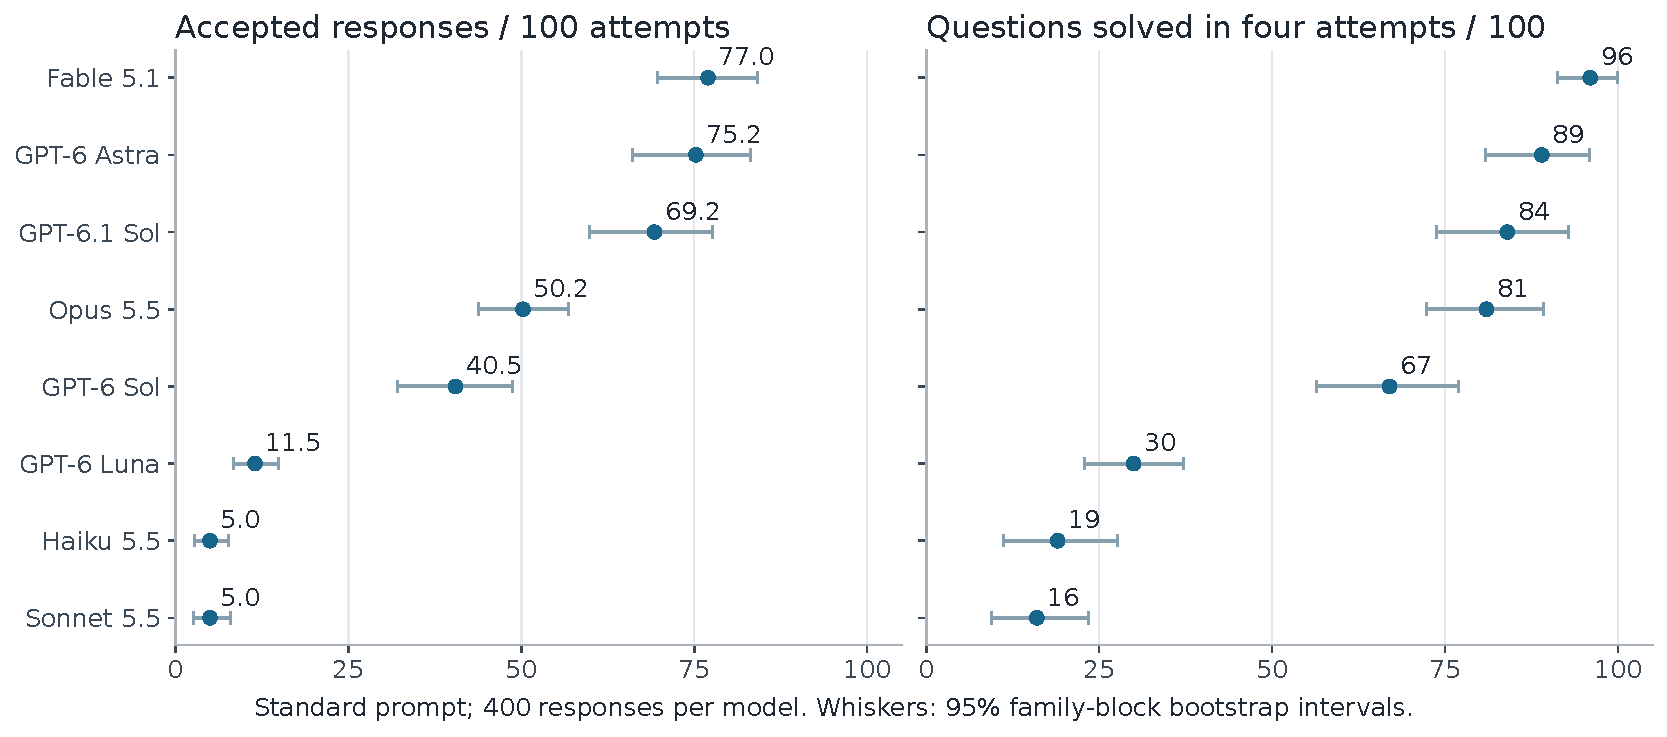
\includegraphics[width=\linewidth]{figures/01_reliability.pdf}
\caption{Two different correctness summaries. Four-attempt coverage must not be confused with per-attempt reliability. Interval widths reflect the family-level resampling analysis.}\label{fig:reliability}
\end{figure}

\subsection{The prompt changes the measured model behavior}
The three instructions produce materially different outcomes (Table~\ref{tab:conditions}). An instruction that helps one model may hurt another. For example, Opus improves from 201/400 accepted under the standard prompt to 284/400 under source concision, a gain of 20.75 percentage points (95\% family-block interval $[14.02,27.39]$; exploratory Holm-adjusted $p<0.001$ across the 24 prompt-yield contrasts). GPT-6.1 Sol and Astra instead lose 11.75 and 12.50 points under source concision, respectively. Their intervals exclude zero and their adjusted $p$-values are approximately 0.027 and 0.012. These are changes in end-to-end protocol acceptance, not isolated measurements of mathematical ability.

The mathematical-compression instruction produces smaller yield differences. All three of Fable, Astra and GPT-6.1 Sol have lower observed acceptance under compression than standard. Their family-bootstrap intervals exclude zero, but the corresponding family-cluster $t$ tests do not survive the full Holm adjustment at 0.05. There is no contradiction: the intervals are unadjusted percentile summaries, whereas the $p$-values use a different small-cluster approximation and multiplicity correction. We report both without treating either as a definitive threshold test.
\begin{table}[htbp]
\centering
\small
\caption{Accepted counts and scheduled yields by prompt. Every cell contains 400 scheduled attempts; truncations and other failures remain in the denominator.}\label{tab:conditions}
\begin{tabular}{lrrr}
\toprule
Model & Standard & Compression & Concision \\
\midrule
Fable 5.1 & 308 (77.00\%) & 283 (70.75\%) & 272 (68.00\%) \\
GPT-6 Astra & 301 (75.25\%) & 269 (67.25\%) & 251 (62.75\%) \\
GPT-6.1 Sol & 277 (69.25\%) & 251 (62.75\%) & 230 (57.50\%) \\
Opus 5.5 & 201 (50.25\%) & 193 (48.25\%) & 284 (71.00\%) \\
GPT-6 Sol & 162 (40.50\%) & 140 (35.00\%) & 138 (34.50\%) \\
GPT-6 Luna & 46 (11.50\%) & 56 (14.00\%) & 47 (11.75\%) \\
Haiku 5.5 & 20 (5.00\%) & 24 (6.00\%) & 13 (3.25\%) \\
Sonnet 5.5 & 20 (5.00\%) & 16 (4.00\%) & 29 (7.25\%) \\
\bottomrule
\end{tabular}
\end{table}
\begin{figure}[htbp]
\centering
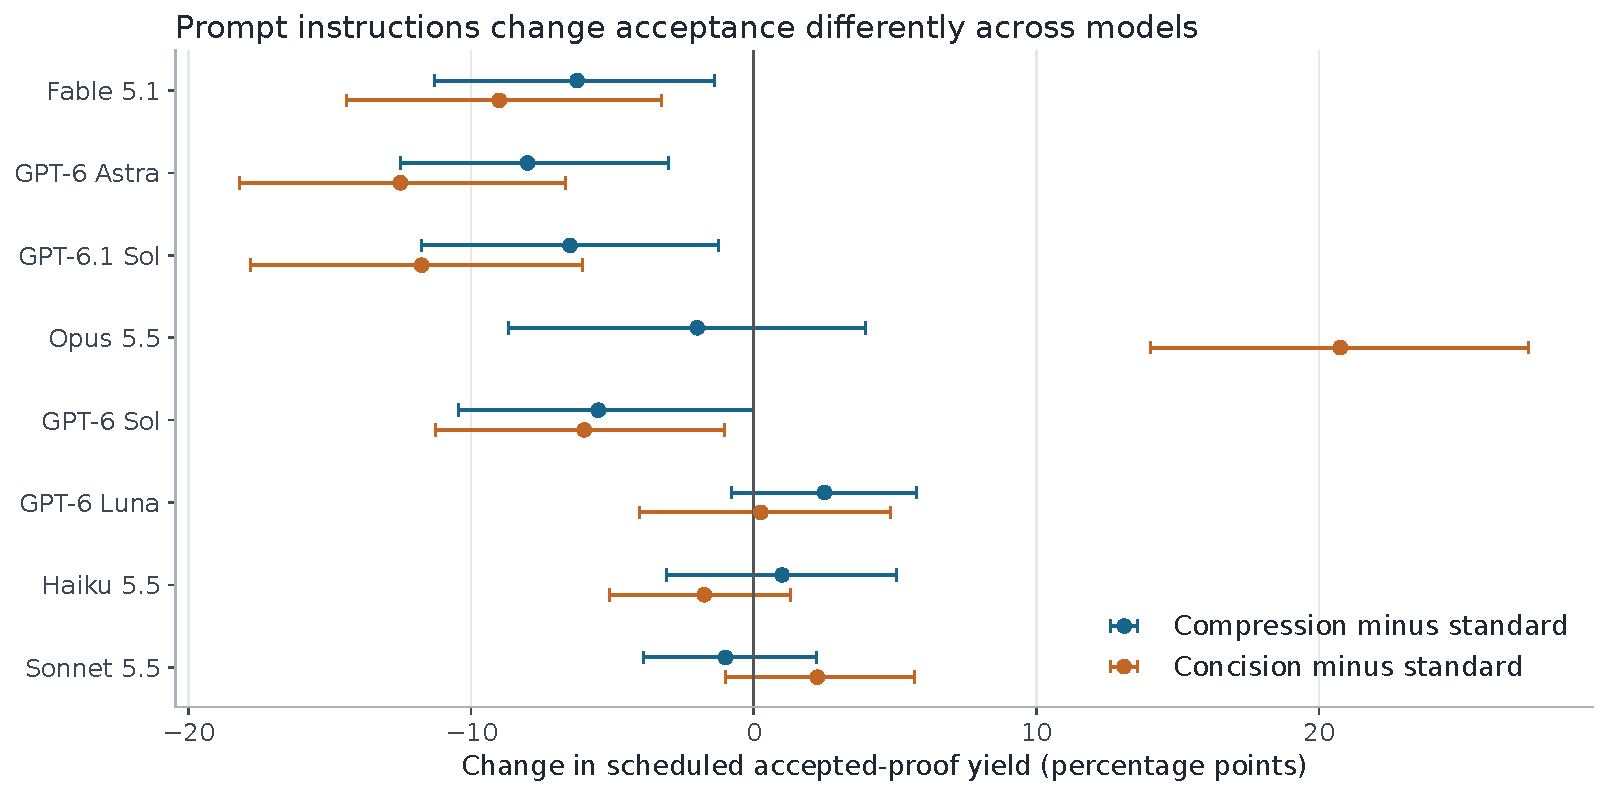
\includegraphics[width=\linewidth]{figures/02_prompt_yield.pdf}
\caption{Paired-question prompt contrasts. Intervals resample the same family blocks across both prompt conditions. They are unadjusted 95\% intervals; multiplicity-adjusted tests are provided separately.}\label{fig:prompt-yield}
\end{figure}

\subsection{Format adherence is a major part of the acceptance outcome}
The failure composition is highly model-dependent (Figure~\ref{fig:outcomes}). Haiku has 1,051 parse failures out of 1,200 scheduled attempts; Sonnet has 1,088. Of these, 970 and 983, respectively, report their first parser error on line 1. An audit of the saved submitted text found frequent headings, prose preceding code, embedded proof wrappers, and, for Sonnet, literal tool-invocation text. A deterministic stratified inspection of ten failures from each model found visible one-term format violations in all ten Haiku and all ten Sonnet examples. This limited sample is not a new automatic classification of every failed proof, and no answers were repaired or regraded.

The frozen adapter removes a single fence or proof wrapper only when it covers the entire response. Prose followed by a code block therefore remains an invalid Lean term. This makes output discipline part of the operational task. It does not imply that every parse failure lacks a mathematically valid argument somewhere inside it. Extracting an alternative candidate and rerunning Lean would define a different evaluation, which was not performed.

The Opus prompt contrast illustrates the distinction. Its standard-prompt parse failures fall from 146/400 to 31/400 under source concision, while accepted proofs rise from 201 to 284. Conditional on escaping the parse-failure category, acceptance is 201/254 (79.13\%) versus 284/369 (76.96\%). That selected comparison is not causal either, but it demonstrates why the overall gain cannot simply be attributed to improved mathematical reasoning. Better compliance with the required output interface is a substantial alternative explanation.
\begin{figure}[htbp]
\centering
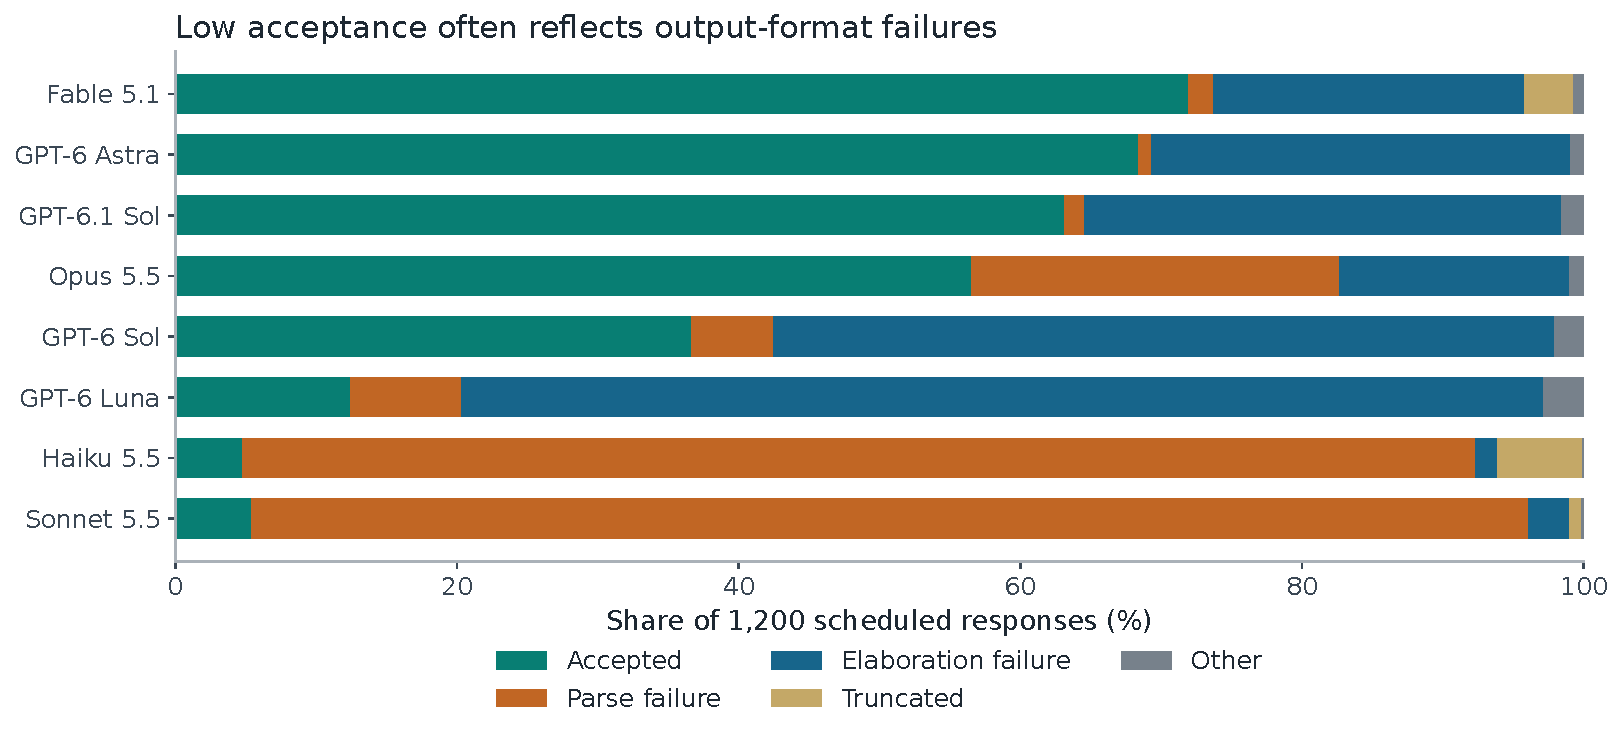
\includegraphics[width=\linewidth]{figures/07_outcomes.pdf}
\caption{All 1,200 scheduled attempts per model in the provider-maximum cohort. ``Other'' combines timeouts, the resource-limit outcome and disallowed axioms. These failures have different meanings and remain distinct in the exported tables.}\label{fig:outcomes}
\end{figure}

\FloatBarrier
\section{Results: compression and source concision}
\label{sec:compression}
\subsection{Benchmark 2: matched-question compression contests}
We compare accepted proofs directly, without dividing by a reference proof's score. For each model pair and prompt, restrict to questions for which both models have at least one valid measurable output. Within each such question, compare every valid response from one model with every valid response from the other. A strictly larger exact $T_0$ earns one point; equality earns half. Average within question, then give every shared question equal weight. This estimates a descriptive conditional win rate over the saved successful responses. It does not give a compression score to a failed proof and does not measure how often a model produces a valid proof in the first place.

Under the compression prompt, Fable wins 60.90\% of these contests against Astra over 77 shared questions (95\% family-block interval $[53.41,69.05]$). Opus wins 67.14\% against Astra over 70 shared questions ($[60.35,73.76]$). Fable versus Opus is unresolved: Fable wins 48.71\% over 78 shared questions ($[40.32,57.17]$). These three comparisons do not use the same question population. They support the stated pairwise conditional descriptions, not a transitive global ranking or a comparison of general reasoning quality. The intervals in this display are descriptive and not simultaneous pairwise confidence bands.

The complete matrix makes the support issue visible (Figure~\ref{fig:pairwise}). Some pairs share very few questions. Most importantly, no question has a measurable compression-prompt proof from all eight models. A pure eight-model ranking on a common compression population is therefore undefined, not zero and not missing because of a plotting inconvenience. The standard and concision instructions have only one and three all-eight shared questions, respectively, which are also inadequate for broad ranking conclusions.
\begin{figure}[htbp]
\centering
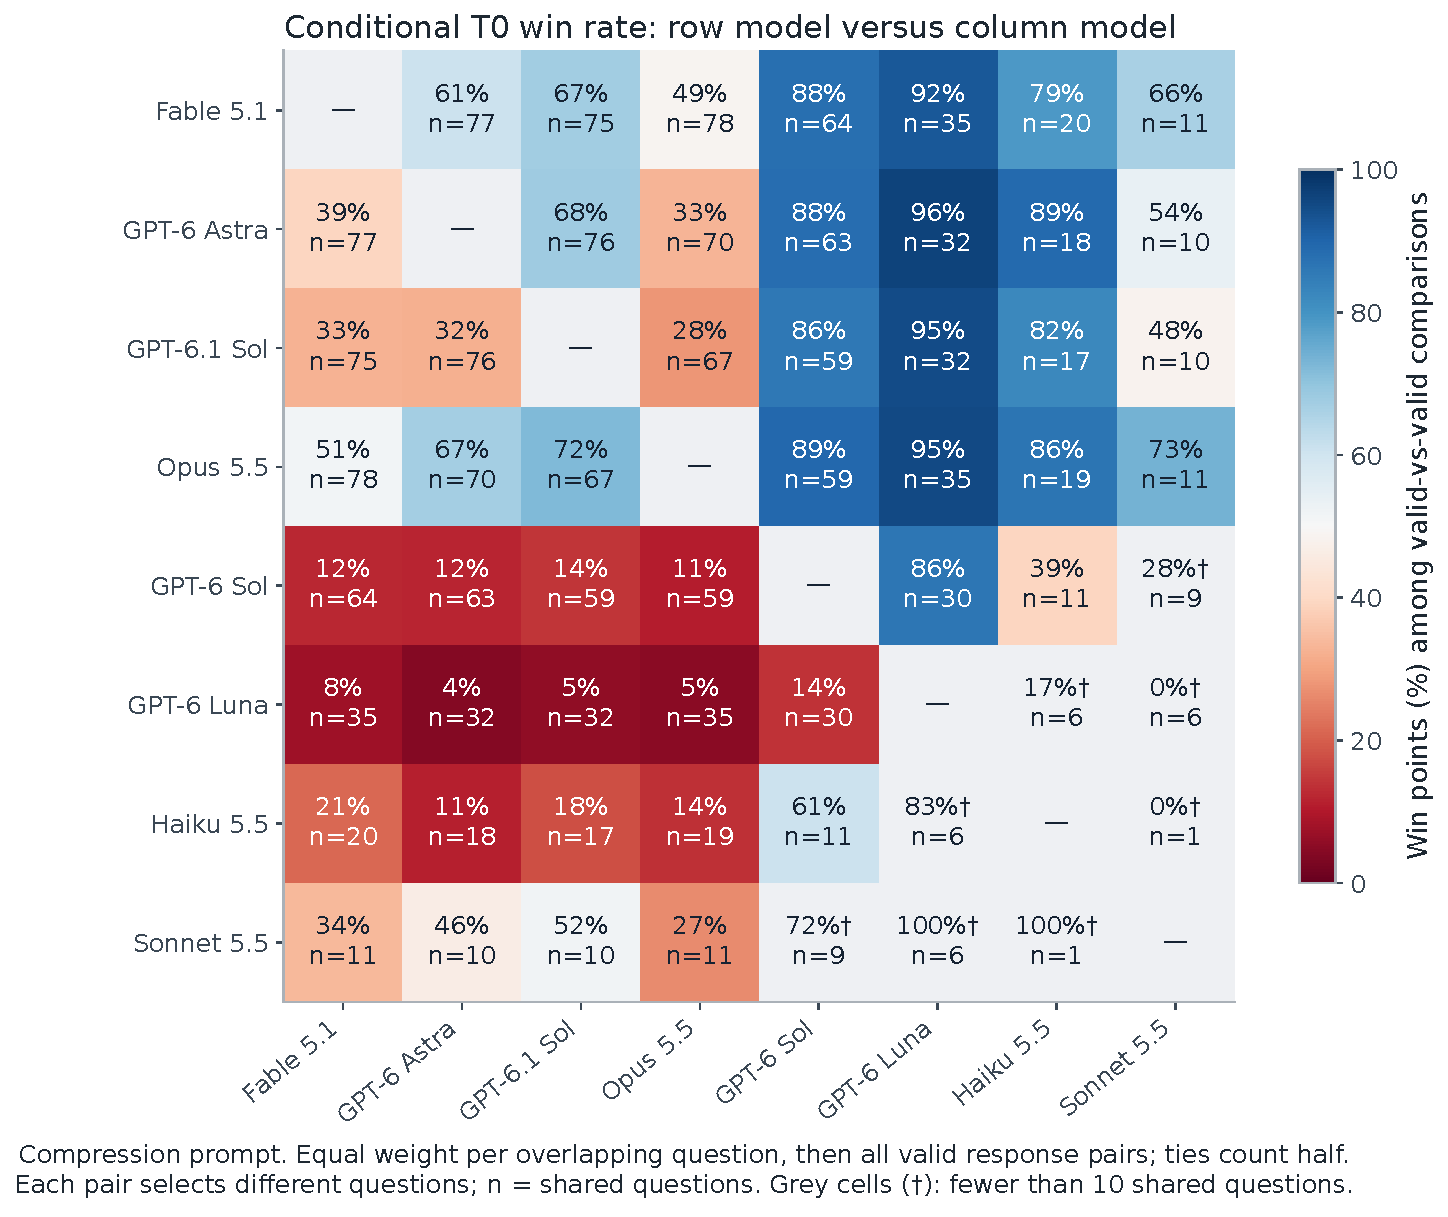
\includegraphics[width=\linewidth]{figures/04_pairwise_compression.pdf}
\caption{Exact conditional $T_0$ comparisons. Rows are the candidate model, columns its opponent. The number in each cell is the count of shared questions. Grey sparse cells retain their descriptive values but are not supported as reliable broad comparisons.}\label{fig:pairwise}
\end{figure}

\subsection{The dashboard's smaller-cohort ranking is a sensitivity view}
The existing dashboard admits models with measurable compression proofs on at least 25 of the 100 questions, then ranks their per-question geometric mean $T_0$ on the common intersection. This selects six models and 23 questions. Fable, Opus and Astra have average ranks of 2.22, 2.35 and 2.57, followed by GPT-6.1 Sol, GPT-6 Sol and Luna. Figure~\ref{fig:ranks} shows uncertainty within that selected support.

This visualization is useful for inspecting a specific comparison. However, both model inclusion and question inclusion depend on observed success. Changing the gate, the model roster or the available samples can change the target population and rank. The intervals condition on that chosen support; they do not account for the selection procedure as though it had been specified before outcomes were observed. We therefore do not headline the 2.22 versus 2.35 difference as a universal model order.
\begin{figure}[htbp]
\centering
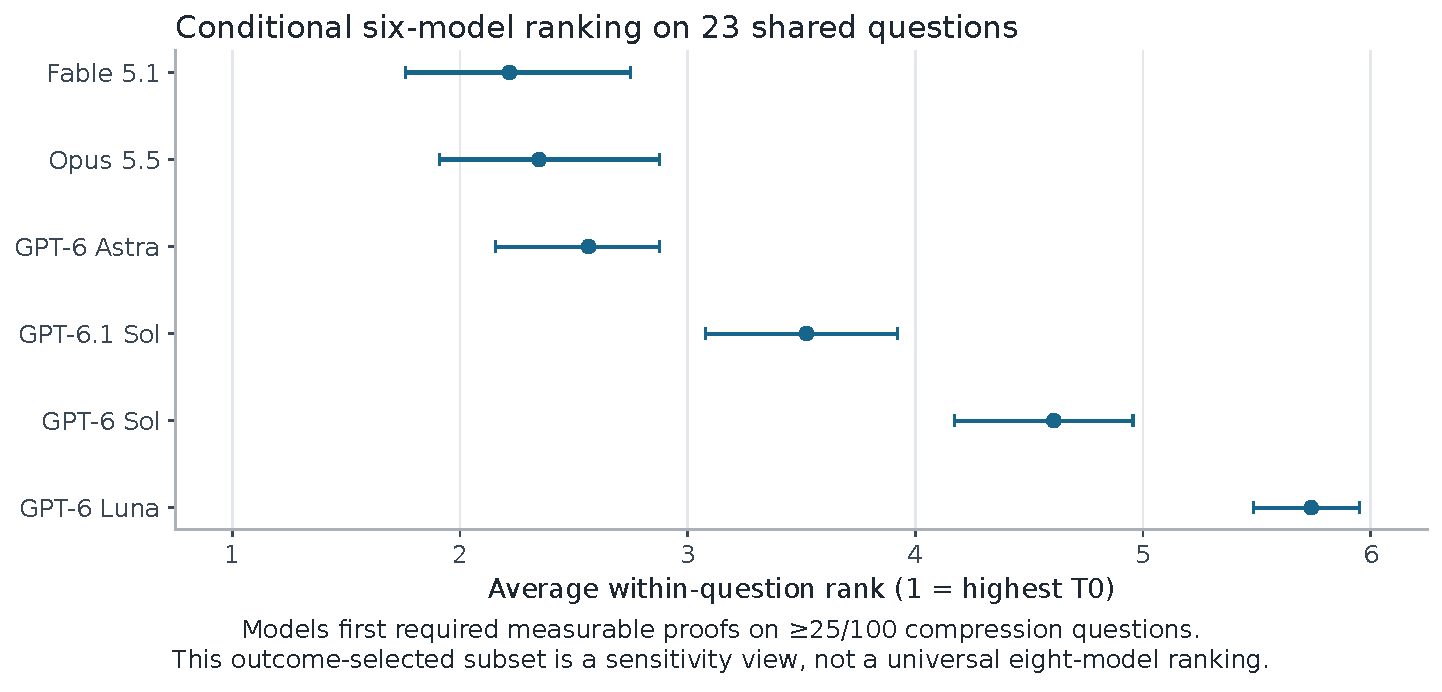
\includegraphics[width=\linewidth]{figures/10_conditional_rank.pdf}
\caption{A faithful statistical rendering of the dashboard's default six-model comparison. Lower average rank denotes higher $T_0$ on the selected 23 shared questions only.}\label{fig:ranks}
\end{figure}

\subsection{Compression prompts shorten accepted proofs, but do not uniformly improve $T_0$}
Among questions with accepted proofs under both prompts, the mathematical-compression instruction often shortens the proof body. Relative to standard, the geometric $W_B$ ratio is 0.65 for Fable, 0.72 for Opus, 0.78 for Astra and 0.80 for GPT-6.1 Sol. Source concision reduces these ratios further to approximately 0.50, 0.61, 0.62 and 0.63. These are conditional paired-question effects, not reductions over all scheduled responses. The number of valid samples also differs between conditions.

The corresponding $T_0$ effects are less straightforward (Figure~\ref{fig:prompt-metrics}). Compression versus standard has point ratios of 1.42 for Fable, 1.21 for Opus, 1.12 for Astra and 1.15 for GPT-6.1 Sol. Some intervals are wide and none of these four compression-versus-standard $T_0$ comparisons survives the full family-cluster Holm analysis at 0.05. Source-concision $T_0$ ratios are more consistently elevated for these models. Sparse Haiku and Sonnet intersections cannot sustain strong conclusions even when an interval is narrow.

The ratio $I_0=W_B/W_S$ is not independent corroboration of source concision. Since $W_S$ is fixed for a question, a within-question change in $\log_2 I_0$ is exactly the same as the change in $\log_2 W_B$. A larger $I_0$ means a longer proof relative to its statement. It should not be silently interpreted as ``better compression'' in a leaderboard aimed at short proofs. Likewise, a normalized blend $J_0$ depends on the selected normalization and cohort; this study does not choose a blend weight to manufacture a winner.
\begin{figure}[htbp]
\centering
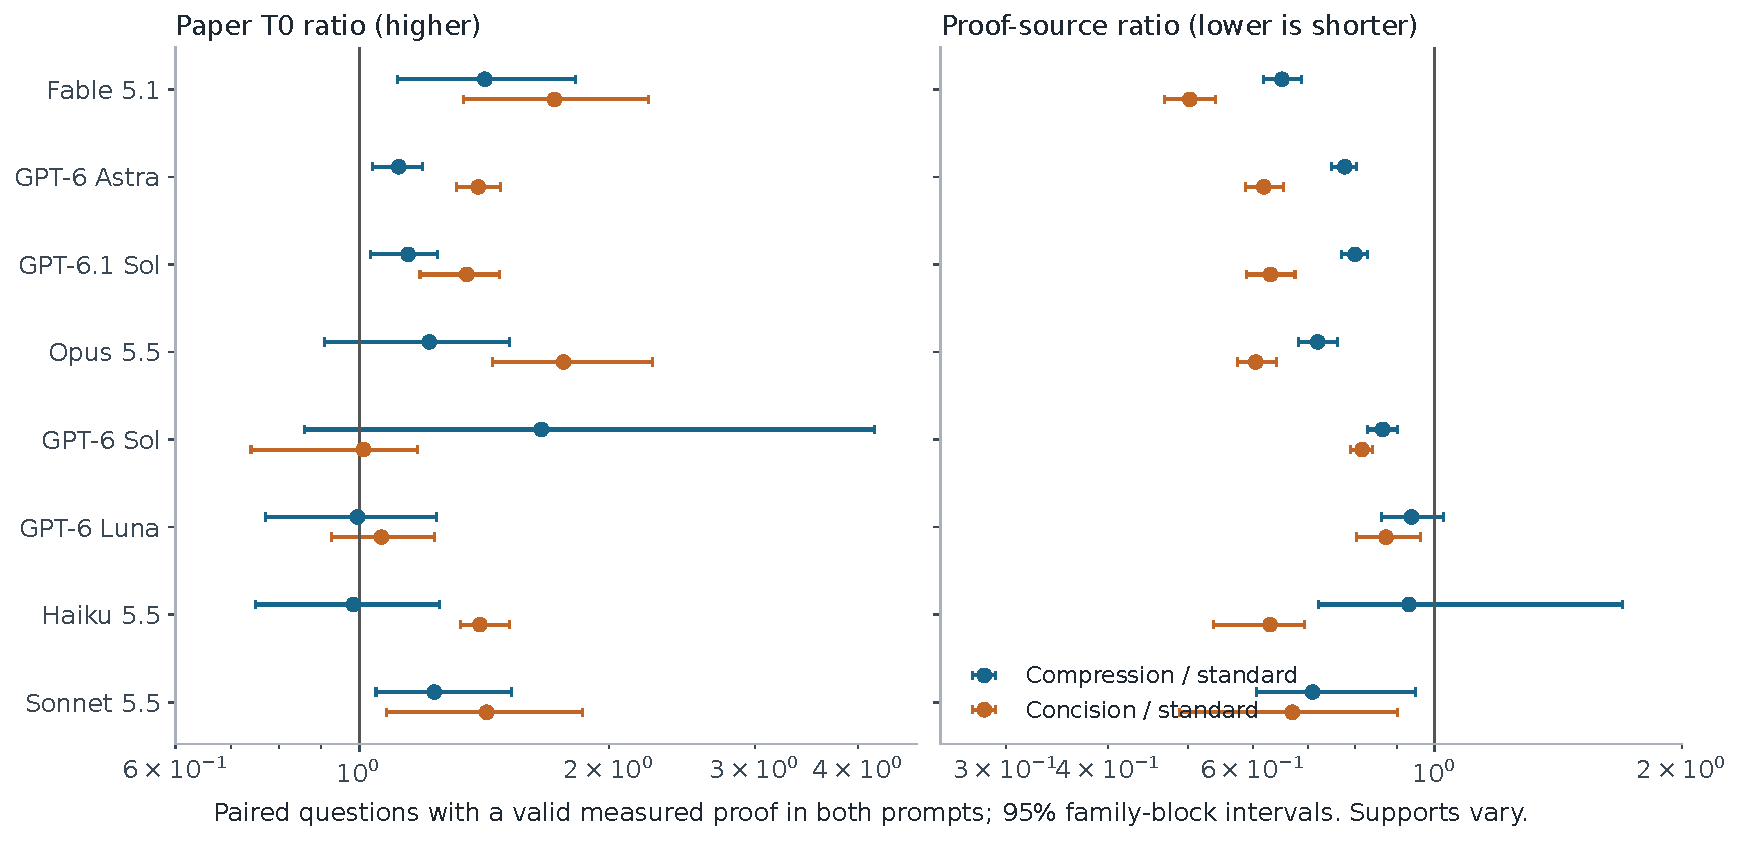
\includegraphics[width=\linewidth]{figures/03_prompt_metrics.pdf}
\caption{Conditional geometric ratios relative to the standard prompt. Each point uses only questions measurable in both relevant conditions. Exact support counts and adjusted tests appear in the supplementary tables. The two panels measure different properties.}\label{fig:prompt-metrics}
\end{figure}

\subsection{Why enormous absolute compression ratios require caution}
A direct mechanism audit finds that the question grouping explains 99.9553\% of the observed sum of squares in $\log_2(U_S+U_B)$ across the provider-maximum accepted outputs. This is a descriptive variance decomposition, not a causal import ablation. It nevertheless explains why comparing raw magnitudes across unrelated questions is misleading. The fixed statement's own numerator is not the main direct contributor: its median share is approximately $1.10\times10^{-7}$ of total $U$, and no measured output exceeds one quarter. Relevant type and library structure also enters through the elaborated proof body.

Pooling all models and prompts within each question, $T_0$ ordering agrees with shorter $W_B$ in 75,603 of 83,774 non-tied valid-output pairs (90.25\%); 304 tied pairs are omitted. Thus higher $T_0$ usually accompanies lower $W_B$ in this pooled comparison. This diagnostic has a different population from the compression-only, cross-model benchmark. Total $U$ is not exactly invariant for any of the 100 questions with multiple measured outputs. Seventy questions have a maximum/minimum $U$ ratio no greater than two, while a few have extreme expansions. We retain these outliers and inspect them instead of deleting them on the basis of their scores.

For OM100-065, a GPT-6 Sol standard proof has $W_B=1{,}669$ and $\log_2 T_0=102.54$; a compression-prompt proof from the same model has $W_B=1{,}198$ and $\log_2 T_0=155.28$. The increase is 52.74 bits, roughly $7.5\times10^{15}$ in the ratio. Only 0.44 bits come from the smaller total source denominator; 52.29 bits come from the numerator. Two references each to the implicitly elaborated \texttt{Real.normedField} and \texttt{Real.normedCommRing} account for essentially all the high proof's expanded body weight. The visible argument takes a reciprocal-limit route; the lower-score proof uses an elementary bound.

For OM100-100, the extreme accepted outputs differ by 25.81 bits of $T_0$. Of this, 24.63 bits arise from larger expanded dependency weight and 1.18 from shorter total source. A single \texttt{Real.instStarOrderedRing} reference contributes 99.999993206\% of the high-score body weight. That name is absent from the written proof and is supplied by elaboration. Fresh independent Python expansion of the four saved proof graphs reproduces all four recorded $U_S$ and $U_B$ values exactly. No arithmetic mismatch was found and no Lean rerun was needed.

These case studies are selected post hoc extremes. They demonstrate a concrete sensitivity of this operational metric; they do not estimate its prevalence or show that a model intentionally gamed the score. Nor do they locate the precise source expression that caused an implicit instance to be inserted. What they do rule out is interpreting every many-order-of-magnitude $T_0$ increase as a proportionate gain in written concision, compression of a fixed semantic payload, or mathematical insight.
\begin{figure}[htbp]
\centering
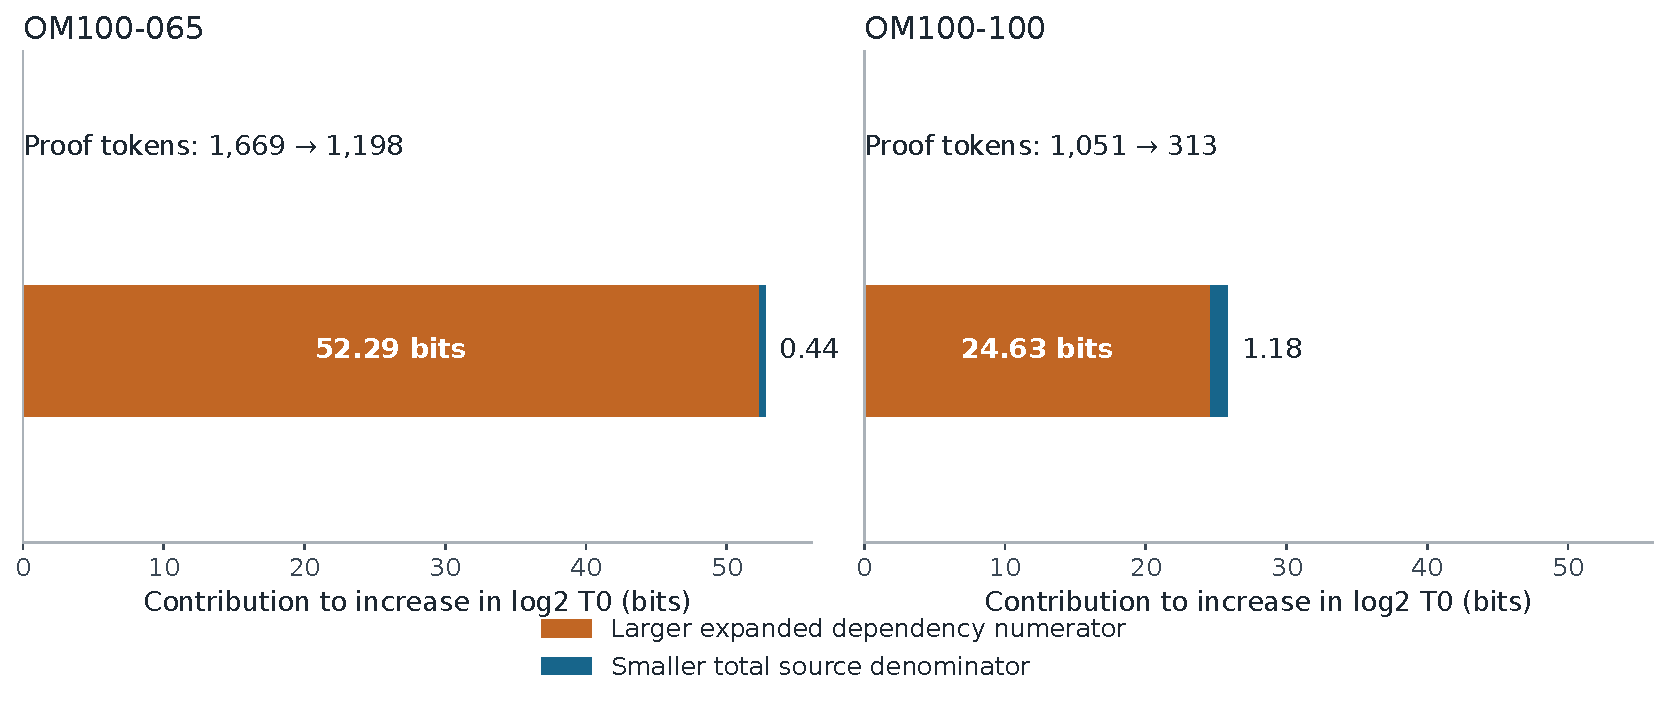
\includegraphics[width=\linewidth]{figures/08_dependency_cases.pdf}
\caption{Exact decomposition $\Delta\log_2 T_0=\Delta\log_2(U_S+U_B)-\Delta\log_2(W_S+W_B)$ for two retained extreme comparisons. Most of each score increase is dependency-numerator growth. These comparisons are diagnostic examples, not randomized prompt effects.}\label{fig:cases}
\end{figure}

\FloatBarrier
\section{Results: the relationship with correctness}
\label{sec:association}
\subsection{Submitted-source length is observable for both outcomes}
Failed proofs have no valid elaborated proof object from which to calculate the primary dependency metric. Giving them $T_0=0$ would combine correctness with compression by fiat. Submitted text length, however, is observable for completed nonempty answers whether or not they are accepted. We use nonwhitespace Unicode character counts for that analysis, not the Lean parser spans $W_B$ that require a valid parsed proof.

Across all 9,477 completed nonempty responses, the raw point-biserial correlation between validity and $\log_2$ source length is $-0.212$. Raw correlation combines differences between questions, models, prompts and response types. After demeaning both variables within question--model--prompt cells, the pooled linear association is a 2.87-percentage-point decrease in acceptance per doubling of source length, with a 95\% family-block interval of $[-5.31,-1.65]$ points (Figure~\ref{fig:length}). This estimator weights observations by their within-cell source-length variation; it is not an equal-question average treatment effect.

Removing parse failures changes the conclusion. Among the remaining 6,809 completed nonempty responses, the analogous within-cell slope is positive: 0.55 points per doubling, with interval $[0.07,0.99]$. The raw correlation is still negative, illustrating the effect of conditioning and within-cell adjustment. Including the 24 nonempty truncated partials instead leaves the main negative association broadly similar. These sensitivities show that ``shorter mathematical proofs are more correct'' is not a justified causal interpretation. The negative association is sensitive to retaining parse-failure responses, which often contain prose.
\begin{figure}[htbp]
\centering
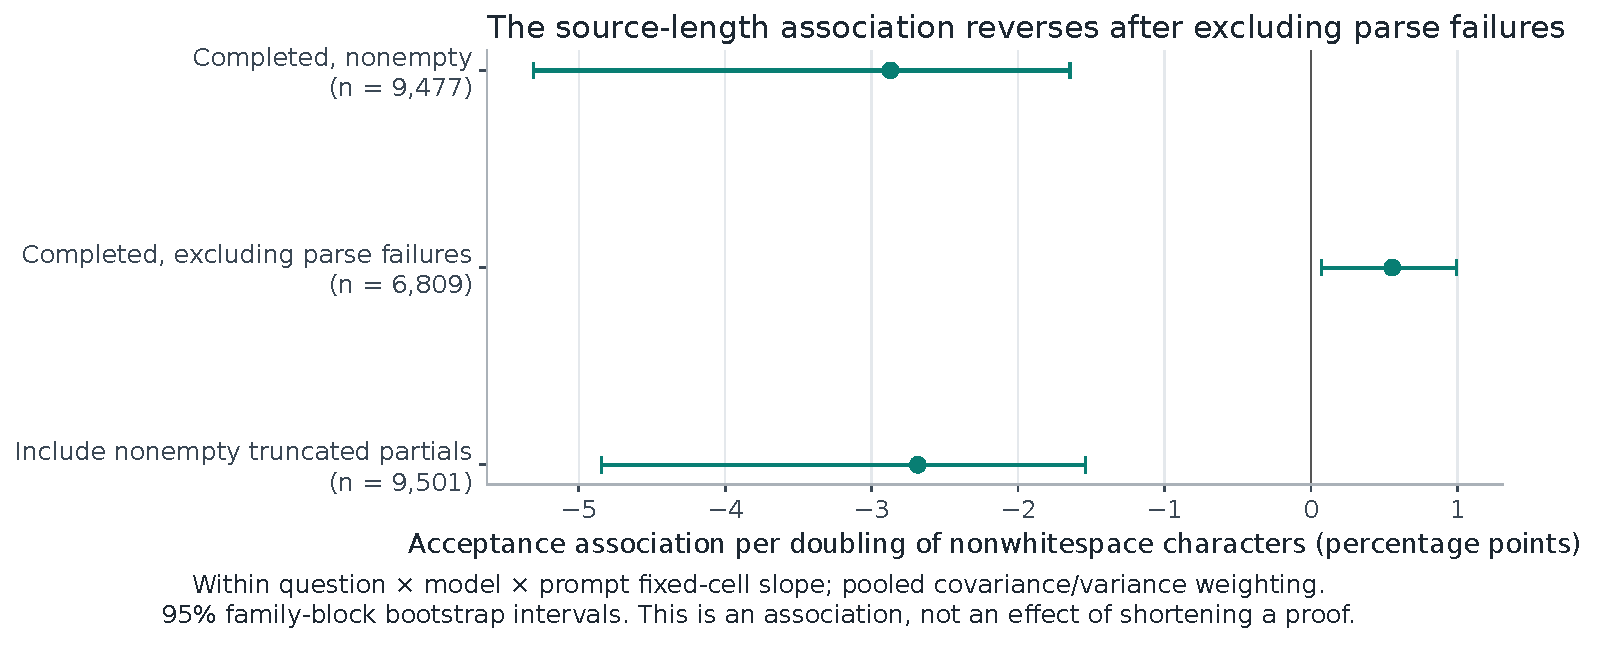
\includegraphics[width=\linewidth]{figures/06_length_association.pdf}
\caption{The response population changes the measured association. This is an observational fixed-cell slope, not evidence that editing an answer to be shorter would change its correctness.}\label{fig:length}
\end{figure}

\subsection{Split-sample compression does not provide clear predictive evidence}
To reduce the circularity of measuring compression and validity from exactly the same successful answers, we use samples 1--2 to estimate the mean log metric among their valid proofs and samples 3--4 to calculate a later scheduled acceptance rate. A model--question--prompt cell enters only if the early half contains a measured proof. We regress the later rate on the early metric with question fixed effects and model-by-prompt controls, using family-clustered uncertainty. We also reverse the two sample halves as a sensitivity check. These are selected, observational regressions; the held-out samples are not a new independently collected test set.

For $\log_2 T_0$, the forward coefficient is 0.76 percentage points per bit (95\% family-cluster interval $[-1.13,2.65]$; 1,216 eligible cells). The reverse coefficient is $-0.23$ points ($[-1.21,0.76]$; 1,197 cells). Both intervals include zero and both tests have Holm-adjusted $p=1$ within the four split-sample metric regressions. The data therefore do not provide clear evidence that higher early $T_0$ predicts later acceptance after these controls. This is not evidence that every possible compression--correctness relationship is absent. Selection, few independent families, measurement sensitivity and the very small number of samples limit the test.

\FloatBarrier
\section{Budget, costs and the earlier cohorts}
\label{sec:budget}
\subsection{The larger-ceiling run changes completion much more than conditional compression}
The 8,192-token cohort has 2,445 accepted proofs, 4,633 completed nonempty submissions and 4,967 truncations. The corresponding provider-maximum counts are 3,831, 9,477 and 123. Scheduled success rises from 25.47\% to 39.91\%, a paired-question increase of 14.44 percentage points, with a 95\% family-block interval of $[11.66,17.19]$. Completion rises from 48.26\% to 98.72\%. Acceptance among completed submissions falls from 52.77\% to 40.42\%, because the completed population expands substantially. Reading only this selected denominator would conceal the improvement in scheduled yield.

The changes differ by model (Figure~\ref{fig:budget}; Table~\ref{tab:budget}). Fable has the largest observed increase across prompts, 53.42 points, followed by Opus at 28.92 points. Their earlier runs had substantial truncation. In contrast, conditional $T_0$ changes on questions solved in both runs are generally near one. Under the compression prompt, the paired geometric rerun/baseline ratios are approximately 1.05 for GPT-6.1 Sol, 1.14 for GPT-6 Sol, 0.93 for Luna, 1.01 for Astra, 1.00 for Opus and 0.98 for Fable. Haiku has no shared measured compression question across runs and Sonnet has only five. Newly solved targets are not assigned a hypothetical baseline compression score.

This is not a causal estimate of giving a model more tokens. The runs contain fresh generations, were collected sequentially, and differ in streaming transport and OpenAI processing tier. The higher ceiling also permits additional reasoning rather than merely a longer final proof. Model-side randomness, service behavior and operational changes cannot be disentangled here. Identical question and prompt hashes support a matched design comparison, not a shared random seed or randomized budget intervention.
\begin{table}[htbp]
\centering
\small
\caption{Matched-question descriptive comparison across all three prompts. Every model has 1,200 scheduled attempts in each run. Generation policies differ beyond the ceiling.}\label{tab:budget}
\begin{tabular}{lrrr}
\toprule
Model & 8,192 yield \% & 128,000 yield \% & Difference pp [95\% CI] \\
\midrule
Fable 5.1 & 18.50 & 71.92 & 53.42 [44.27, 62.66] \\
GPT-6 Astra & 60.75 & 68.42 & 7.67 [3.30, 12.66] \\
GPT-6.1 Sol & 58.25 & 63.17 & 4.92 [-0.65, 10.86] \\
Opus 5.5 & 27.58 & 56.50 & 28.92 [20.63, 37.42] \\
GPT-6 Sol & 28.92 & 36.67 & 7.75 [3.28, 12.07] \\
GPT-6 Luna & 5.17 & 12.42 & 7.25 [4.81, 9.86] \\
Haiku 5.5 & 0.08 & 4.75 & 4.67 [3.56, 5.79] \\
Sonnet 5.5 & 4.50 & 5.42 & 0.92 [-0.07, 1.86] \\
\bottomrule
\end{tabular}
\end{table}
\begin{figure}[htbp]
\centering
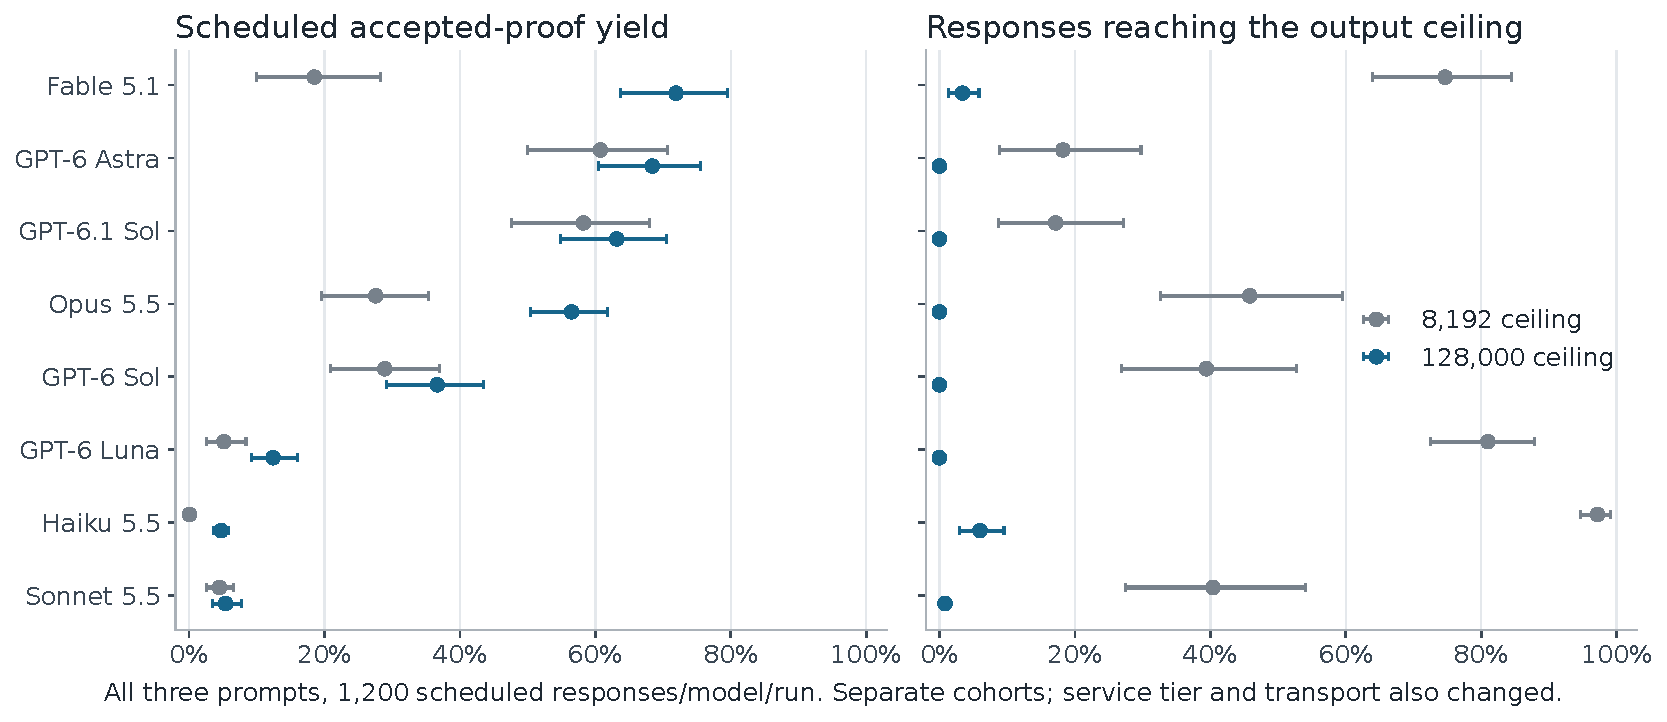
\includegraphics[width=\linewidth]{figures/05_budget_comparison.pdf}
\caption{Accepted-proof yield and native-ceiling truncation across the two substantive cohorts. Each interval resamples source-result families, retaining all attempts.}\label{fig:budget}
\end{figure}

\subsection{Costs are recorded-response estimates, not invoices}
The initial substantive run's recorded-response API estimate is \$1,848.44; the provider-maximum rerun's is \$4,369.72. The latter is approximately 2.36 times the former. The initial report retains an as-of VM compute subtotal of \$56.82 (14 October 2026, 19:38:21 UTC); the rerun's closed allocation estimate is \$59.33. Summing the priced API components, historical initial compute subtotal and closed rerun compute estimate gives approximately \$6,334.31 across the two substantive runs, but this is not a complete expenditure total. Seven original requests in the first run and 30 in the rerun have unresolved charges. Storage, public-IP, network, tax and credit adjustments are also outside these compute estimates. Smoke-stage costs are not reconstructed from unavailable legacy provenance.

Within the provider-maximum cohort, recorded API cost per accepted proof ranges widely (Figure~\ref{fig:cost}). This quotient includes the model's priced failed responses, but not the unresolved original-request charges or shared cloud cost. It is not the price of guaranteeing a solution to an arbitrary question: success probabilities are heterogeneous, repeated sampling may not be independent, and targets unsolved in all four attempts remain. A low quotient for a model with low coverage does not make it an interchangeable substitute for a higher-coverage model.

OpenAI estimates use the recorded delivered tier and frozen cache/output prices; Anthropic has no separately reported reasoning-token counter in this evidence, which is left missing rather than zero. Reasoning already belongs to billed output where reported and is not charged twice. Generation wall times include service, concurrency and transport effects; verification times additionally involve two physical CPU families. We provide distributions for transparency but make no controlled latency or compute-efficiency claim. The task's six rerun VMs were deallocated, allocation intervals were closed from observed lifecycle records, and the dedicated resource group was confirmed deleted after local hash-verified backups.
\begin{figure}[htbp]
\centering
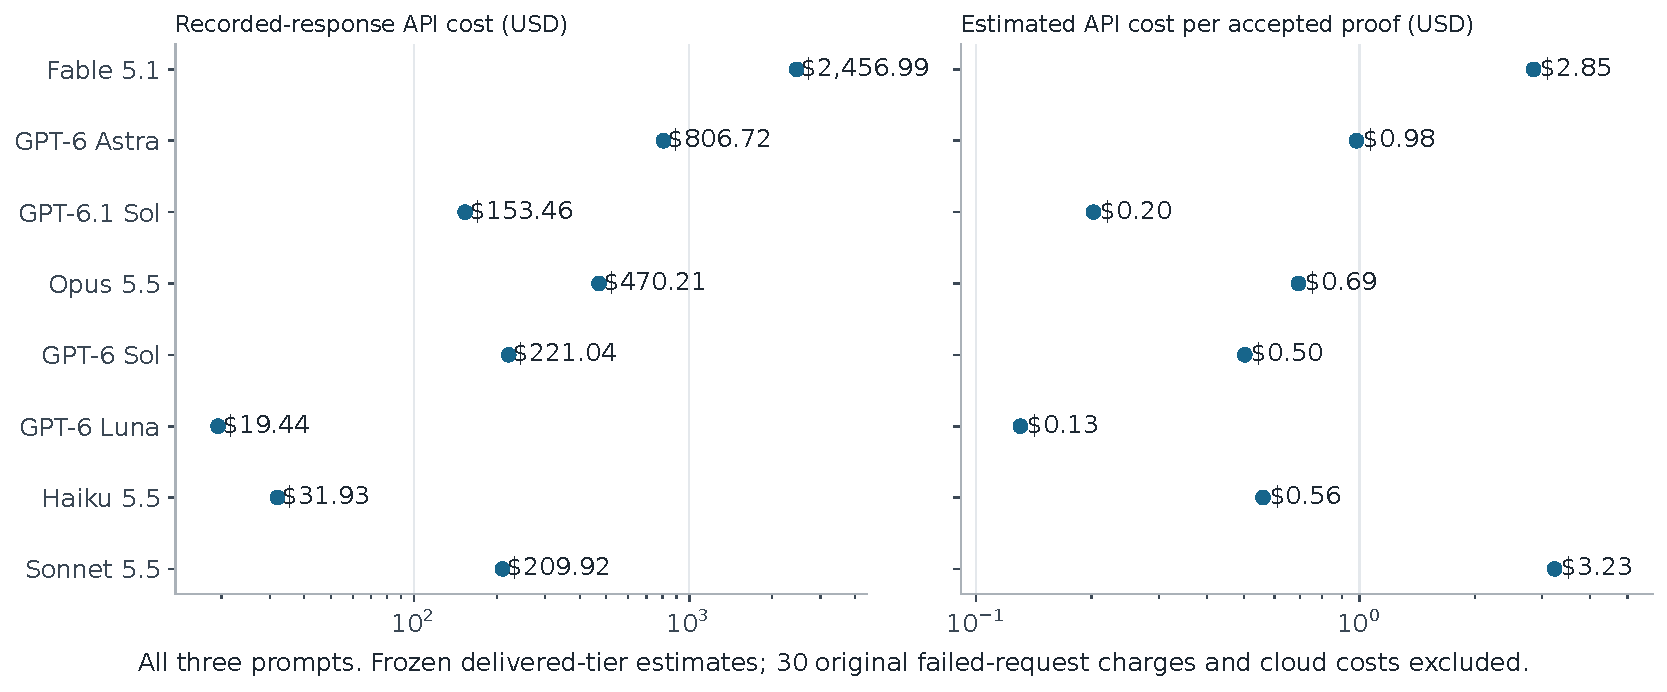
\includegraphics[width=\linewidth]{figures/09_costs.pdf}
\caption{Costs across all three prompts in the provider-maximum cohort. The log axes compare scales; points and labels give the actual estimates. These figures exclude shared VM costs and unresolved original-request charges.}\label{fig:cost}
\end{figure}

\subsection{The smoke test served an engineering purpose}
The ten-question smoke suite has 960 scheduled attempts, 609 accepted proofs and 602 measurable accepted proofs. Its simpler tasks, earlier Lean/library environment, response adapter and resource limits differ from OM100. Its high acceptance cannot validate the substantive task selection or be pooled with the 19,200 OM100 attempts. Seven accepted smoke proofs have unavailable compression metrics and remain accepted with missing metrics. The accompanying data package includes all model-by-prompt smoke summaries as descriptive engineering evidence.

\FloatBarrier
\section{Interpretation, limitations and recommendations}
\label{sec:discussion}
\paragraph{What has been measured.}
The strongest supported claims concern formal acceptance under a declared environment, observed submitted-source concision, and a weighted dependency-expansion ratio. These are valuable, reproducible properties. None is a direct observation of a model's internal reasoning process. A short proof can use automation or a powerful premise; a high expansion ratio can reward an implicit typeclass hierarchy. These possibilities are not merely theoretical in this dataset: saved accepted proof graphs exhibit them.

\paragraph{Selection changes the meaning of a comparison.}
There are three successive selections: a curated set of public component lemmas, completed responses, and valid measurable proofs. Each answers a different question. Scheduled yield retains every planned attempt and is the appropriate main reliability endpoint. Completed-response acceptance diagnoses quality among delivered texts. Conditional compression describes successful proofs on an explicitly shared support. It cannot recover a missing compression value for an invalid proof, and it can favor models that solve a narrow subset of questions. Reporting all three is more informative than silently dropping failures or awarding them an arbitrary zero ratio.

\paragraph{The corpus is not certified unseen.}
The selected source developments were publicly released recently, but the mathematical statements may have older antecedents, and the upstream repository itself contains artifacts produced by an internal OpenAI model. The exact training exposure of each evaluated model is unknown. Reference-informed premise retrieval further shapes the supplied context. Equal prompts ensure equal observed inputs, but do not demonstrate equal prior exposure or eliminate a potential provenance asymmetry. The study should be described as an evaluation on 100 selected public Lean lemmas, not as solving 100 new open research problems.

\paragraph{Dependence and researcher choices constrain inference.}
The 100 targets come from 19 result families and 92 source files. Nearby lemmas share machinery, and the four attempts are not four independent mathematical tasks. Family-block resampling and clustered regressions account for one important dependence level, but 19 clusters are few. The percentile intervals, CR1 correction and $t$ reference distribution do not guarantee calibrated population coverage. The corpus was not randomly sampled, many analyses were chosen after results were visible, and the headline social summaries are post hoc. Holm correction limits a declared set of exploratory comparisons, not every analysis decision made during the project.

\paragraph{Operational boundaries remain part of the result.}
The strict one-term format, frozen response adapter, time and memory budgets, allowed axioms, dependency boundary and source-token definition all affect outcomes. A timeout is not a mathematical counterexample; a prose-plus-code response is not an accepted submission under this protocol even if some embedded proof might work. No salvage parser or additional proof search was introduced after seeing the failures. Regrading such responses would require a separately named and uniformly applied evaluation. The present paper preserves every original outcome.

\paragraph{A better next study would separate the questions more sharply.}
For reliability, use a locked set of targets with independently calibrated difficulty, documented exposure risk and family-separated development/test partitions. If the aim is compression conditional on solving, choose a common task support using an independent calibration stage, rather than selecting the final intersection from the same outputs being ranked. For representation metrics, report proof-body source size beside dependency expansion, identify the largest contributing implicit instances, and evaluate sensitivity to a declared alternative boundary. If semantic abstraction is the construct of interest, expert review or targeted structural measurements are needed; source length or $T_0$ alone does not establish it.

For budget effects, randomize or interleave generation policies while holding processing tier, transport, model endpoint and sampling procedure fixed. For format robustness, preregister a single extraction policy and report both strict interface compliance and any separately evaluated salvage condition. For statistics, choose the small set of estimands and multiplicity families before generating the confirmatory test set, and budget for enough independent theorem families rather than simply more samples of the same lemmas.

\section{Conclusion}
The completed corpus supports a rigorous but limited comparison of model-generated Lean proofs. The provider-maximum run produced 3,831 accepted proofs from 9,600 scheduled attempts, with much less truncation than the 8,192-token cohort. Strong observed proof coverage does not imply a resolved compression ranking: the all-eight compression intersection is empty, and leading conditional comparisons depend on their shared questions. Compression and concision instructions often shorten accepted source, but acceptance can fall, and format adherence can dominate a model-specific gain. Extreme $T_0$ changes can be driven by implicit library expansion. The appropriate conclusion is to measure correctness, source concision and dependency expansion together, with explicit populations and uncertainty, rather than treating any one as a universal proxy for mathematical reasoning.

\paragraph{Data, code and authorship note.}
This technical report was prepared with AI assistance from frozen evaluation artifacts and reproducible statistical scripts. It is a draft for review, not a peer-reviewed publication. No human authorship, affiliation, preregistration or independent blinded assessment is claimed. The accompanying bundle contains an executed analysis notebook, derived tables, figure sources, short benchmark definitions and source hashes. Raw provider captures and full proof graphs remain in the retained local evaluation archives; API credentials and hidden reasoning are not included in this report bundle. The evaluation source archive was pushed before this post-hoc analysis; the present paper and social drafts have not been publicly posted.

\begin{thebibliography}{9}
\bibitem{compression} V. Aksenov, E. Bodnia, M. H. Freedman, and M. Mulligan. \emph{Compression is all you need: Modeling Mathematics}. arXiv:2603.20396, 2026, version 1, especially Sections 3 and 5. \url{https://arxiv.org/abs/2603.20396}.
\bibitem{openaimath} OpenAI. \emph{math: mathematical manuscripts and supporting proof artifacts}. Repository snapshot \texttt{adc7f1241b42e322a6451854ab7e4b4c146bf78a}, README and source files, accessed October 2026. \url{https://github.com/openai/math/tree/adc7f1241b42e322a6451854ab7e4b4c146bf78a}.
\bibitem{humaneval} M. Chen et al. \emph{Evaluating Large Language Models Trained on Code}. arXiv:2107.03374, 2021, Section 2.1 and Appendix A. \url{https://arxiv.org/abs/2107.03374}.
\bibitem{cluster} A. C. Cameron and D. L. Miller. A Practitioner's Guide to Cluster-Robust Inference. \emph{Journal of Human Resources} 50(2):317--372, 2015. \url{https://cameron.econ.ucdavis.edu/research/Cameron_Miller_JHR_2015.pdf}.
\bibitem{leandojo} K. Yang et al. \emph{LeanDojo: Theorem Proving with Retrieval-Augmented Language Models}. arXiv:2306.15626, 2023. \url{https://arxiv.org/abs/2306.15626}.
\end{thebibliography}

\appendix
\section{Complete prompt-contrast tables}
The tables below retain the scheduled-yield denominator and the selected paired-question compression denominator separately. All intervals are unadjusted 95\% family-block bootstrap intervals. The ``Holm'' column for yield controls the declared 24 prompt-yield contrasts. For the metric table, complete adjusted tests, exact numerators and denominators, sample counts and decomposition terms are supplied in the machine-readable tables. Sparse intersections are descriptive; an apparently tight interval from only a few families does not establish robust generalization.
\small
\begin{longtable}{llrrr}
\caption{All scheduled-yield prompt contrasts (percentage points).}\label{tab:all-yield}\\
\toprule Model & Comparison & Estimate & 95\% interval & Holm $p$\\\midrule\endfirsthead
\toprule Model & Comparison & Estimate & 95\% interval & Holm $p$\\\midrule\endhead
Fable 5.1 & Compression--Standard & -6.25 & [-11.29, -1.38] & 0.486 \\
Fable 5.1 & Concision--Standard & -9.00 & [-14.39, -3.27] & 0.123 \\
Fable 5.1 & Compression--Concision & +2.75 & [-2.27, +8.17] & 1.000 \\
GPT-6 Astra & Compression--Standard & -8.00 & [-12.50, -3.02] & 0.091 \\
GPT-6 Astra & Concision--Standard & -12.50 & [-18.18, -6.65] & 0.012 \\
GPT-6 Astra & Compression--Concision & +4.50 & [-0.25, +9.34] & 1.000 \\
GPT-6.1 Sol & Compression--Standard & -6.50 & [-11.75, -1.25] & 0.493 \\
GPT-6.1 Sol & Concision--Standard & -11.75 & [-17.82, -6.06] & 0.027 \\
GPT-6.1 Sol & Compression--Concision & +5.25 & [-0.50, +11.09] & 1.000 \\
Opus 5.5 & Compression--Standard & -2.00 & [-8.66, +3.96] & 1.000 \\
Opus 5.5 & Concision--Standard & +20.75 & [+14.02, +27.39] & $<0.001$ \\
Opus 5.5 & Compression--Concision & -22.75 & [-27.87, -17.90] & $<0.001$ \\
GPT-6 Sol & Compression--Standard & -5.50 & [-10.46, +0.00] & 0.886 \\
GPT-6 Sol & Concision--Standard & -6.00 & [-11.25, -1.03] & 0.611 \\
GPT-6 Sol & Compression--Concision & +0.50 & [-5.15, +6.18] & 1.000 \\
GPT-6 Luna & Compression--Standard & +2.50 & [-0.77, +5.75] & 1.000 \\
GPT-6 Luna & Concision--Standard & +0.25 & [-4.04, +4.85] & 1.000 \\
GPT-6 Luna & Compression--Concision & +2.25 & [-1.99, +6.31] & 1.000 \\
Haiku 5.5 & Compression--Standard & +1.00 & [-3.09, +5.05] & 1.000 \\
Haiku 5.5 & Concision--Standard & -1.75 & [-5.11, +1.30] & 1.000 \\
Haiku 5.5 & Compression--Concision & +2.75 & [-0.28, +5.79] & 1.000 \\
Sonnet 5.5 & Compression--Standard & -1.00 & [-3.91, +2.21] & 1.000 \\
Sonnet 5.5 & Concision--Standard & +2.25 & [-0.99, +5.69] & 1.000 \\
Sonnet 5.5 & Compression--Concision & -3.25 & [-7.41, +0.24] & 1.000 \\
\bottomrule\end{longtable}
\begin{longtable}{llrrll}
\caption{Conditional proof-metric ratios. Ratios above one indicate larger values in the first prompt. $n$ counts paired questions; $G$ counts represented families.}\label{tab:all-metrics}\\
\toprule Model & Comparison & $n$ & $G$ & $T_0$ ratio [95\% CI] & $W_B$ ratio [95\% CI]\\\midrule\endfirsthead
\toprule Model & Comparison & $n$ & $G$ & $T_0$ ratio [95\% CI] & $W_B$ ratio [95\% CI]\\\midrule\endhead
Fable 5.1 & Comp/Std & 89 & 19 & 1.42 [1.11, 1.82] & 0.65 [0.62, 0.69] \\
Fable 5.1 & Conc/Std & 90 & 19 & 1.72 [1.33, 2.23] & 0.50 [0.47, 0.54] \\
Fable 5.1 & Comp/Conc & 86 & 19 & 0.83 [0.79, 0.87] & 1.27 [1.23, 1.32] \\
GPT-6 Astra & Comp/Std & 83 & 18 & 1.12 [1.04, 1.19] & 0.78 [0.75, 0.80] \\
GPT-6 Astra & Conc/Std & 81 & 19 & 1.39 [1.31, 1.48] & 0.62 [0.59, 0.65] \\
GPT-6 Astra & Comp/Conc & 78 & 19 & 0.79 [0.72, 0.84] & 1.26 [1.21, 1.31] \\
GPT-6.1 Sol & Comp/Std & 75 & 18 & 1.15 [1.03, 1.24] & 0.80 [0.77, 0.83] \\
GPT-6.1 Sol & Conc/Std & 74 & 19 & 1.35 [1.18, 1.48] & 0.63 [0.59, 0.68] \\
GPT-6.1 Sol & Comp/Conc & 72 & 18 & 0.86 [0.82, 0.90] & 1.25 [1.19, 1.30] \\
Opus 5.5 & Comp/Std & 71 & 18 & 1.21 [0.91, 1.52] & 0.72 [0.68, 0.76] \\
Opus 5.5 & Conc/Std & 79 & 19 & 1.76 [1.45, 2.26] & 0.61 [0.57, 0.64] \\
Opus 5.5 & Comp/Conc & 79 & 18 & 0.71 [0.45, 0.94] & 1.18 [1.14, 1.22] \\
GPT-6 Sol & Comp/Std & 57 & 18 & 1.66 [0.86, 4.18] & 0.86 [0.83, 0.90] \\
GPT-6 Sol & Conc/Std & 51 & 18 & 1.01 [0.74, 1.17] & 0.82 [0.79, 0.84] \\
GPT-6 Sol & Comp/Conc & 51 & 18 & 1.05 [0.89, 1.37] & 1.05 [1.00, 1.10] \\
GPT-6 Luna & Comp/Std & 20 & 14 & 1.00 [0.77, 1.24] & 0.94 [0.86, 1.02] \\
GPT-6 Luna & Conc/Std & 15 & 13 & 1.06 [0.93, 1.23] & 0.87 [0.80, 0.96] \\
GPT-6 Luna & Comp/Conc & 17 & 12 & 0.93 [0.78, 1.10] & 1.04 [0.97, 1.12] \\
Haiku 5.5 & Comp/Std & 4 & 4 & 0.98 [0.75, 1.25] & 0.93 [0.72, 1.69] \\
Haiku 5.5 & Conc/Std & 4 & 4 & 1.40 [1.33, 1.52] & 0.63 [0.54, 0.69] \\
Haiku 5.5 & Comp/Conc & 6 & 6 & 0.95 [0.88, 1.05] & 1.07 [0.97, 1.17] \\
Sonnet 5.5 & Comp/Std & 4 & 3 & 1.23 [1.05, 1.53] & 0.71 [0.61, 0.95] \\
Sonnet 5.5 & Conc/Std & 6 & 5 & 1.42 [1.08, 1.86] & 0.67 [0.49, 0.90] \\
Sonnet 5.5 & Comp/Conc & 5 & 4 & 0.91 [0.75, 0.99] & 1.17 [1.04, 1.39] \\
\bottomrule\end{longtable}\normalsize
\section{An explicitly supplemental joint contest}
\label{app:joint}
The original evaluation proposal rejected a combined quality score. To answer the practical request for easily communicated comparisons, we also examined a new \emph{post-hoc descriptive contest}, kept separate from the scientific primary endpoints. Fix the eight-model roster and the compression prompt. Select a question uniformly, a rival uniformly from the other seven models, and one of the four saved responses from each. A valid proof beats a failed response; two valid proofs are ordered by exact $T_0$; equality or two failures split a point. Average all 16 response pairs within each question. This score combines reliability and compression and must never be called the paper's compression metric.

For a pair of models with question-specific valid fractions $p_A,p_B$, and conditional valid-pair win rate $w$, the score has the exact decomposition
\[
S_{AB}=\tfrac12+\tfrac12(p_A-p_B)+p_Ap_B(w-\tfrac12).
\]
The last term is zero when no valid pair exists. Thus every model receives 50 on a question where all models fail; 50 is not an adequacy threshold. The score also changes if the competitor roster changes. Table~\ref{tab:joint} reports the components so that a reliability advantage cannot be disguised as a pure compression advantage. This supplemental construction is not used in the two scientific benchmark cards.
\begin{table}[htbp]
\centering
\small
\caption{New joint contest, with baseline 50 points plus reliability and metric terms. The last two columns describe contest mass, not independent sample counts.}\label{tab:joint}
\begin{tabular}{lrrrrr}
\toprule
Model & Joint points & Reliability & Metric term & Both fail \% & Both valid \% \\
\midrule
Fable 5.1 & 72.91 & +18.43 & +4.48 & 21.8 & 26.4 \\
GPT-6 Astra & 68.62 & +16.43 & +2.19 & 25.0 & 26.6 \\
GPT-6.1 Sol & 62.58 & +13.86 & -1.27 & 27.9 & 25.7 \\
Opus 5.5 & 59.70 & +5.57 & +4.13 & 34.5 & 19.9 \\
GPT-6 Sol & 42.44 & -2.00 & -5.56 & 42.4 & 16.4 \\
GPT-6 Luna & 32.76 & -14.00 & -3.24 & 51.2 & 7.2 \\
Haiku 5.5 & 30.67 & -18.57 & -0.76 & 53.5 & 2.7 \\
Sonnet 5.5 & 30.32 & -19.71 & +0.04 & 54.9 & 2.3 \\
\bottomrule
\end{tabular}
\end{table}

\section{Family and domain support}
The four supplied selection groups each contain 25 questions, but the 19 source-result families have unequal sizes. This motivates reporting equal-question estimates with family dependence, rather than treating each generated response as an independent theorem. Figure~\ref{fig:families} displays standard-prompt acceptance by family. The derived data include the complete 100-question metadata and model-by-question outcomes; no unmeasured difficulty label is treated as a calibrated covariate.
\begin{figure}[htbp]
\centering
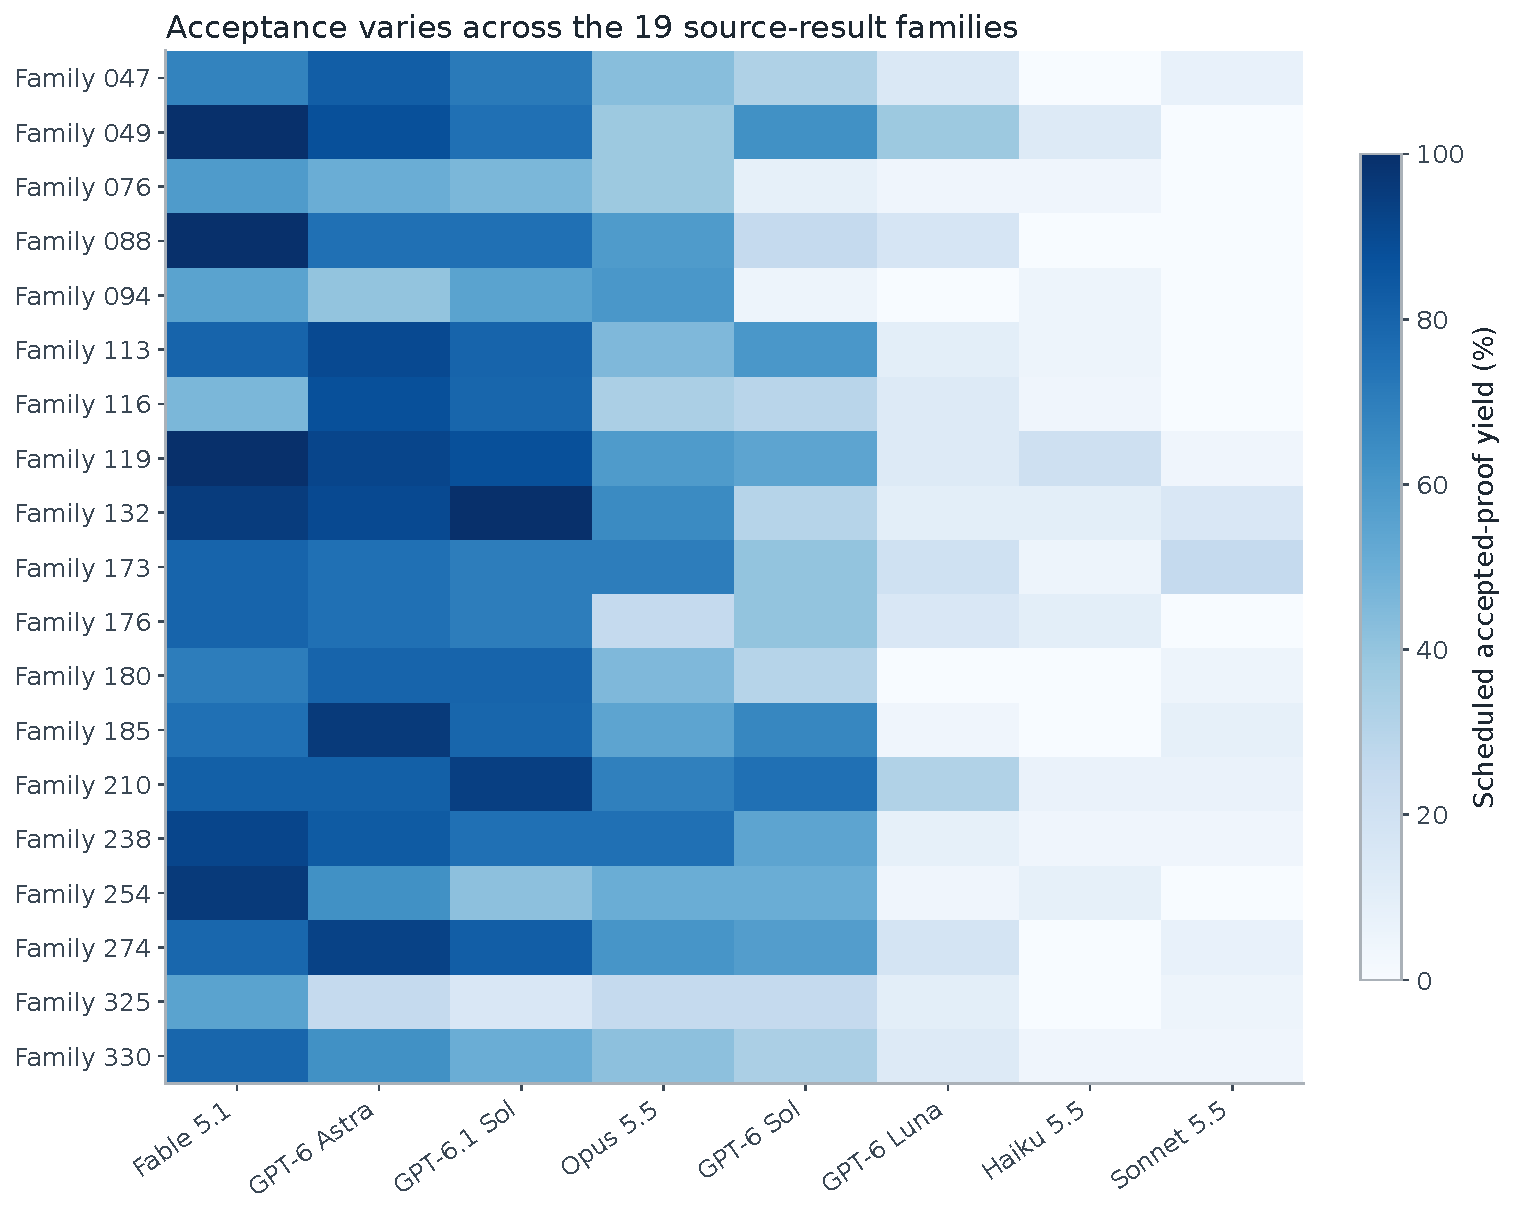
\includegraphics[width=\linewidth]{figures/11_family_heatmap.pdf}
\caption{Standard-prompt acceptance by model and source-result family. The matrix is descriptive; family sizes range from two to seven questions.}\label{fig:families}
\end{figure}
\begin{table}[htbp]
\centering
\small
\caption{Composition of the selected 100 questions. IDs and titles identify source developments; they are not independent validation of novelty or difficulty.}\label{tab:families}
\begin{tabular}{llrp{8.2cm}}
\toprule
Family & Selection group & $n$ & Upstream family title \\
\midrule
047 & algebra & 7 & Complex counterexamples to cancellation and affine fibrations \\
049 & algebra & 2 & A stable-coordinate counterexample in four variables \\
076 & analysis & 6 & Ultraflat real Littlewood polynomials \\
088 & analysis & 3 & Petty's projection-volume conjecture and simplex counterexamples \\
094 & analysis & 5 & Subpolynomial dimension reduction in $L\_p$ \\
113 & combinatorics & 5 & Approximate counting and the perfect-matching entropy conjecture \\
116 & cs\_probability & 6 & Uniform identity testing for noncommutative formulas \\
119 & cs\_probability & 6 & The Courtade--Kumar and Hellinger conjectures \\
132 & combinatorics & 5 & A counterexample to the quadratic sensitivity conjecture \\
173 & combinatorics & 5 & Seymour's second-neighborhood conjecture \\
176 & combinatorics & 5 & The second Kahn--Kalai conjecture \\
180 & combinatorics & 5 & Barnette's Hamiltonian-cycle conjecture \\
185 & algebra & 6 & Counterexamples to infinite matroid intersection and packing/covering \\
210 & algebra & 4 & Foulkes' conjecture for sixth powers and quadratic stabilization \\
238 & cs\_probability & 6 & Optimal logarithmic mixing of the Thorp shuffle \\
254 & algebra & 6 & Classifying spaces and geometric obstructions for Artin groups \\
274 & cs\_probability & 7 & Moore's parity conjecture for $\textbackslash{}mathrm{QAC}^0$ \\
325 & analysis & 5 & The complete Crouzeix conjecture \\
330 & analysis & 6 & A negative answer to Kalton's Lipschitz-free approximation question \\
\bottomrule
\end{tabular}
\end{table}
\clearpage
\section{Exact prompts and operational provenance}
\small
\label{app:exact-prompts}

The common system message was:
\begin{verbatim}
You are completing a Lean theorem in the supplied fixed environment.
Return exactly one Lean proof term that fills <PROOF> in the target.
A tactic proof beginning with "by" is allowed.
Prove the exact target using its stated assumptions and the supplied imports.
Do not return Markdown fences, prose, a replacement declaration, imports,
top-level commands, new axioms, sorry, admit, or custom metaprogramming.
Ordinary local have and let expressions are allowed.
\end{verbatim}
The three condition instructions follow. Line wrapping here is typographic; the archived specification retains the exact original bytes.

\paragraph{Standard.}
\begin{verbatim}
Produce a correct Lean proof of the target.
\end{verbatim}
\paragraph{Mathematical compression.}
\begin{verbatim}
Produce a correct Lean proof in the most mathematically compressed form you
can. Use suitable existing definitions and lemmas, and factor repeated
reasoning locally, to express the argument compactly. Avoid irrelevant
reasoning or artificial expansion.
\end{verbatim}
\paragraph{Source concision.}
\begin{verbatim}
Produce a correct Lean proof using as few Lean source tokens as possible.
\end{verbatim}

The smoke cohort preceded OM100 development. Initial OM100 manifests were frozen on 14 October 2026 UTC, with completion recorded at 19:46 UTC. The separate provider-maximum manifests were frozen on 15 October at 02:38 UTC; final validation passed at 04:42 UTC. Six checker VMs were confirmed deallocated at approximately 04:51 UTC, and the task resource group was confirmed absent at 04:56:17 UTC. These operational events changed neither proof outcomes nor source metrics. The rerun verification fleet comprised six VMs with 384 vCPUs and 3 TiB of RAM in aggregate; per-proof limits remained fixed. A reporting-test hard link changed manifest inode metadata but not file bytes, triggering a generation-supervisor integrity guard. Already dispatched streams finished naturally; no provider request was terminated to finish sooner. Exactly 30 original failures (11 terminal provider failures, including three provider timeouts, and 19 pre-stream disconnects) received separately reviewed one-use replacement releases. Original failure evidence and unknown charges were preserved. Completed saved responses were never repeated. Complete text-only terminal responses could be reconciled from saved stream evidence without executing returned tools or making a new request.

Short provenance prefixes identify retained full hashes: OpenAI source commit \texttt{adc7f1241b42}; Lean commit \texttt{5045d0056413}; Mathlib commit \texttt{d13f23b723b8}; frozen Python evaluator \texttt{958bc7676b5f}; Lean evaluator \texttt{2ff87da0a2eb}; scorer \texttt{cdd3c7f0d364}; prompt policy \texttt{e768e4350173}; v2 image \texttt{3889fa8d304a}; reference index \texttt{5c44821af7cc}; provider-maximum comparison data \texttt{4ddf80101317}; and post hoc analysis specification \texttt{2415d3f0b3d0}. Full values, manifests, raw-response and verification evidence, source-span policies, and the preserved runtime archive are recorded in the companion provenance files. Source-only rebuilding is not claimed to reproduce the image digest bit for bit.

\end{document}
